\documentclass[UTF8]{ctexart}
\usepackage{amsmath}
\usepackage{diagbox}
\usepackage{textcomp}
\usepackage{graphicx}
\usepackage{float}
\begin{document}

%\pagestyle{plain}
\linespread{1.4}
\title{\vspace{-5em}\heiti弦振动实验报告\vspace{-2.5em}}
\date{}
\maketitle
\begin{center}
{\fangsong 徐浩博\quad 基科01\quad2020010108}
\end{center}

\subsubsection*{摘要}
\kaishu\normalsize 本实验旨在通过对在周期性正弦激励下的弦线受迫振动并在特定频率下产生驻波的现象的观察和分析,使我对弦振动的相关知识,如弦振动方程、弦末端固定时的边界条件和反射特性、形成驻波的条件等,具有了更深刻的认识。其次,通过实验的测量、分析以及不确定的计算,我初步掌握了进行物理实验的步骤和基本方法,了解到了实验过程中是如何进行测量、记录、排除干扰等各项工作的。最后,通过对数据的测量与分析,我还初步掌握了如何进行误差分析与不确定度计算。
\subsubsection*{关键词:弦振动;受迫振动;驻波;边界条件;反射现象;弦振动方程\vspace{1.5em}}


\section{实验仪器}
\songti 信号发生器与双通道示波器\par 驱动线圈与接收线圈\par 6根不同线密度的弦线\par 砝码钩(质量为$200g$)及5个质量为$200g$的砝码\par 仪器基座台及其上固定的蝶形螺母、弦码、定位柱和两个定滑轮等\par


\section{实验原理}
\subsubsection*{A) 弦振动方程}
\begin{figure}[H]\centering\kaishu{
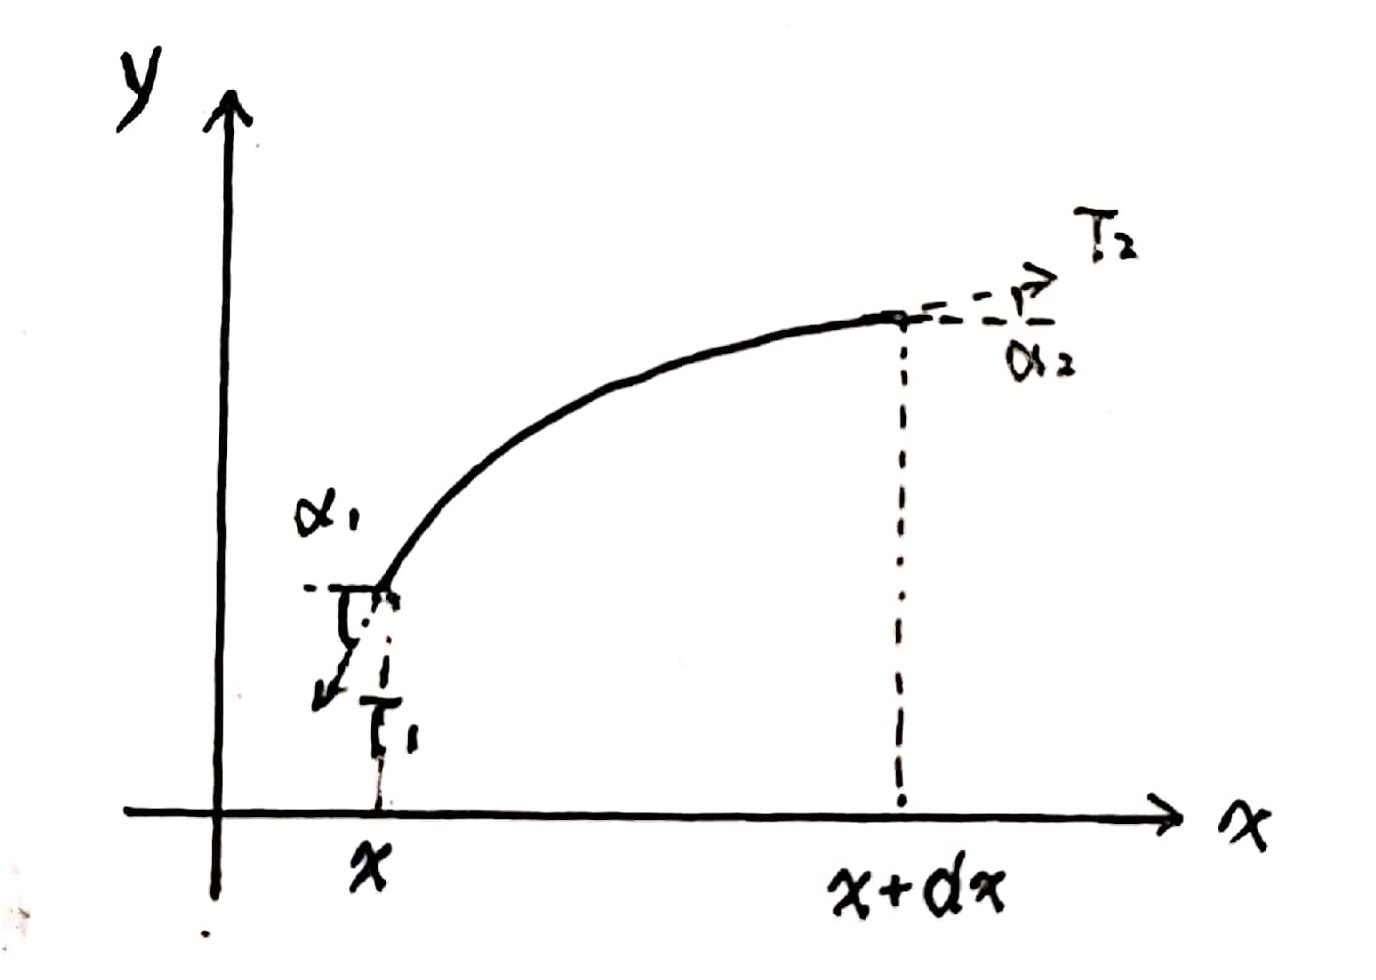
\includegraphics[scale=0.15]{theory.jpg}
\caption{一小段弦线受力分析}}
\end{figure}
\songti 如图,设弦线密度为$\rho$,对$(x,x+dx)$之间一小段弦线进行受力分析,有方程:
\begin{equation}
T_2\cos\alpha_2-T_1\cos\alpha_1 = 0\\
\end{equation}
\begin{equation}
T_2\sin\alpha_2-T_1\sin\alpha_1 = \rho
{\frac{\partial {}^2y}{\partial t^2}} \mathrm{d}x
\end{equation}
\songti 取近似 $\cos\alpha_1 \approx \cos\alpha_2 \approx 1$,$\sin\alpha_1 \approx \tan\alpha_1 \approx \displaystyle{\frac{\partial y}{\partial x}}\Big|_x$,$\sin\alpha_2 \approx \tan\alpha_2 \approx \displaystyle{\frac{\partial y}{\partial x}}\Big|_{x+\mathrm{d}x}$,可解得:
\begin{equation}
\displaystyle{\frac{\partial ^2y}{\partial t^2}-\frac{T}{\rho}\frac{\partial ^2y}{\partial x^2} = 0}
\end{equation}
\songti 此为弦振动方程. 记\begin{equation}\label{velocity}\displaystyle{v=\sqrt{\frac{T}{\rho}}}\end{equation}则弦振动方程的通解可表示为$\displaystyle{y = f(vt\pm x)}$.

\subsubsection*{B) 正弦激励下的弦线末端边界条件和振动反射现象}
\songti 设原来的波为$y^+ = A_1e^{i(\omega t+kx+\phi_1)}$,反射波为$y^-=A_2e^{i(\omega t-kx+\phi_2)}$,设边界位置$x = 0$和$x = L$,由边界位置固定,有$y^+(t,x = 0)+y^-(t,x = 0) = 0$和$y^+(t,x = L)+y^-(t,x = L) = 0$,由此推出$y = -2A_1e^{\phi_1}(e^{ikx}-e^{-ikx})$,设$\phi_1 = 0$,并取$y$的实部得:
\begin{equation}
y = A_1\sin(kx)\sin(\omega t)
\end{equation}


\subsubsection*{C) 正弦激励下弦线的驻波现象}
\songti 由方程$y = A_1\sin(kx)\sin(\omega t)$可知,若在边界$x = L$处有$\sin(kx) = 0$,则在两个边界处,反射后叠加时原波与反射波处于波谷,由此可以产生驻波。综合以上,形成驻波的条件为$kL = n\pi (n = 1,2,\cdots)$. 在由$v = f\lambda$,可以得到:
\begin{equation}
\displaystyle{f = \frac{n}{2L}v = \frac{n}{2L}\sqrt{\frac{T}{\rho}}}\label{f}
\end{equation}


\section{实验步骤及数据处理}
\songti \textbf{从公式${f = \frac{n}{2L}\sqrt{\frac{T}{\rho}}}$知,$f$仅与$n$、$L$、$T$、$\rho$四个变量有关,因此我们将采用控制变量法,使得四个变量分别变化,验证$f$与它们的关系. 最后由(4)式和(6)式两个等式分别得出的弦上振动传播速度$v$进行对比验证.}\par
\songti 选用合适弦线进行下列实验时,均要将弦的一端穿过蝶形螺母的小孔,另一端与跨过两个定滑轮的细线相连,线的另一端悬吊砝码钩,可根据实验需要增减砝码钩上的砝码. 
\songti 进行下列试验前,需要打开信号发生器,并将其置于正弦输出,同时将输出信号的峰峰值$V_{pp}$调节至合适的数值,如$4 - 6V$,并将初始的频率降至$10^1 - 10^2Hz$的数量级. 打开示波器后,同时打开$CH1$和$CH2$两个通道,并调节水平偏转因子和$CH1$垂直偏转因子,以屏幕上出现清晰的若干波形为宜.\par
\songti 在寻找特定条件下的共振频率时,可将理论数据代入${f = \frac{n}{2L}\sqrt{\frac{T}{\rho}}}$以估量出此条件下共振频率大致的数值,在估值附近上下调节发生器信号频率,寻找$CH2$正弦图像稳定、清晰且振幅最大的信号频率.\par



\subsubsection*{A) 探究$f$与$n$的关系}
采用控制变量法,需要控制$L$、$T$、$\rho$的数值. 控制两个弦码的间距为$L = 50.00cm$,并在砝码钩上放置4个砝码,使得弦上张力为$F = 9.800N$. 用正弦波对弦进行激励,对$n = 1, 2, 3, 4, 5$五种情况下较粗的5\#和6\#弦线形成驻波时的共振频率进行测量.\par
由公式${f = \frac{n}{2L}\sqrt{\frac{T}{\rho}}},$计算对$f$与$n$拟合出的截距为0的直线理论斜率$k_0$,直线斜率应为$k_0=\frac{1}{2L}\sqrt{\frac{T}{\rho}}$.

\paragraph{对于6\#弦线的数据分析如下:}
\begin{center}
{\kaishu 表1\quad6\#弦线共振频率$f$与半波数$n$关系实验数据表}
\begin{tabular}{|c|c|c|c|c|c|}
\hline
	{半波数\tiny\quad\normalsize$n$}&1&2&3&4&5\\
\hline
	{共振频率$f/Hz$}&{31.91}&{65.55}&{98.31}&{132.33}&{167.87}\\
\hline
\end{tabular}
\end{center}
\par 对6\#弦线半波数$n = 1 - 5$时共振频率$f$进行测量,所得数据如表1所示. 对此组数据利用Excel程序的linest函数对$f$和$n$做截距为0的最小二乘法直线拟合,设直线斜率为$k$,利用Excel程序的tinv函数计算$p = 0.95$时的$t$因子,可得到:\par
\begin{center}\begin{tabular}{r l}
{斜率}& {$k=33.21109Hz$}\\
{斜率标准偏差}& {$s_k=0.187831Hz$}\\
{t因子}& {$t_{0.95,4}=2.776445$}\\
{斜率不确定度}& {$U_k=t_{0.95,4}\times s_k = 0.521503Hz$}
\end{tabular}\end{center}
因此,f、n拟合得出的直线斜率为$k=(33.2\pm0.5)Hz$\par
\begin{figure}[H]\centering\kaishu{
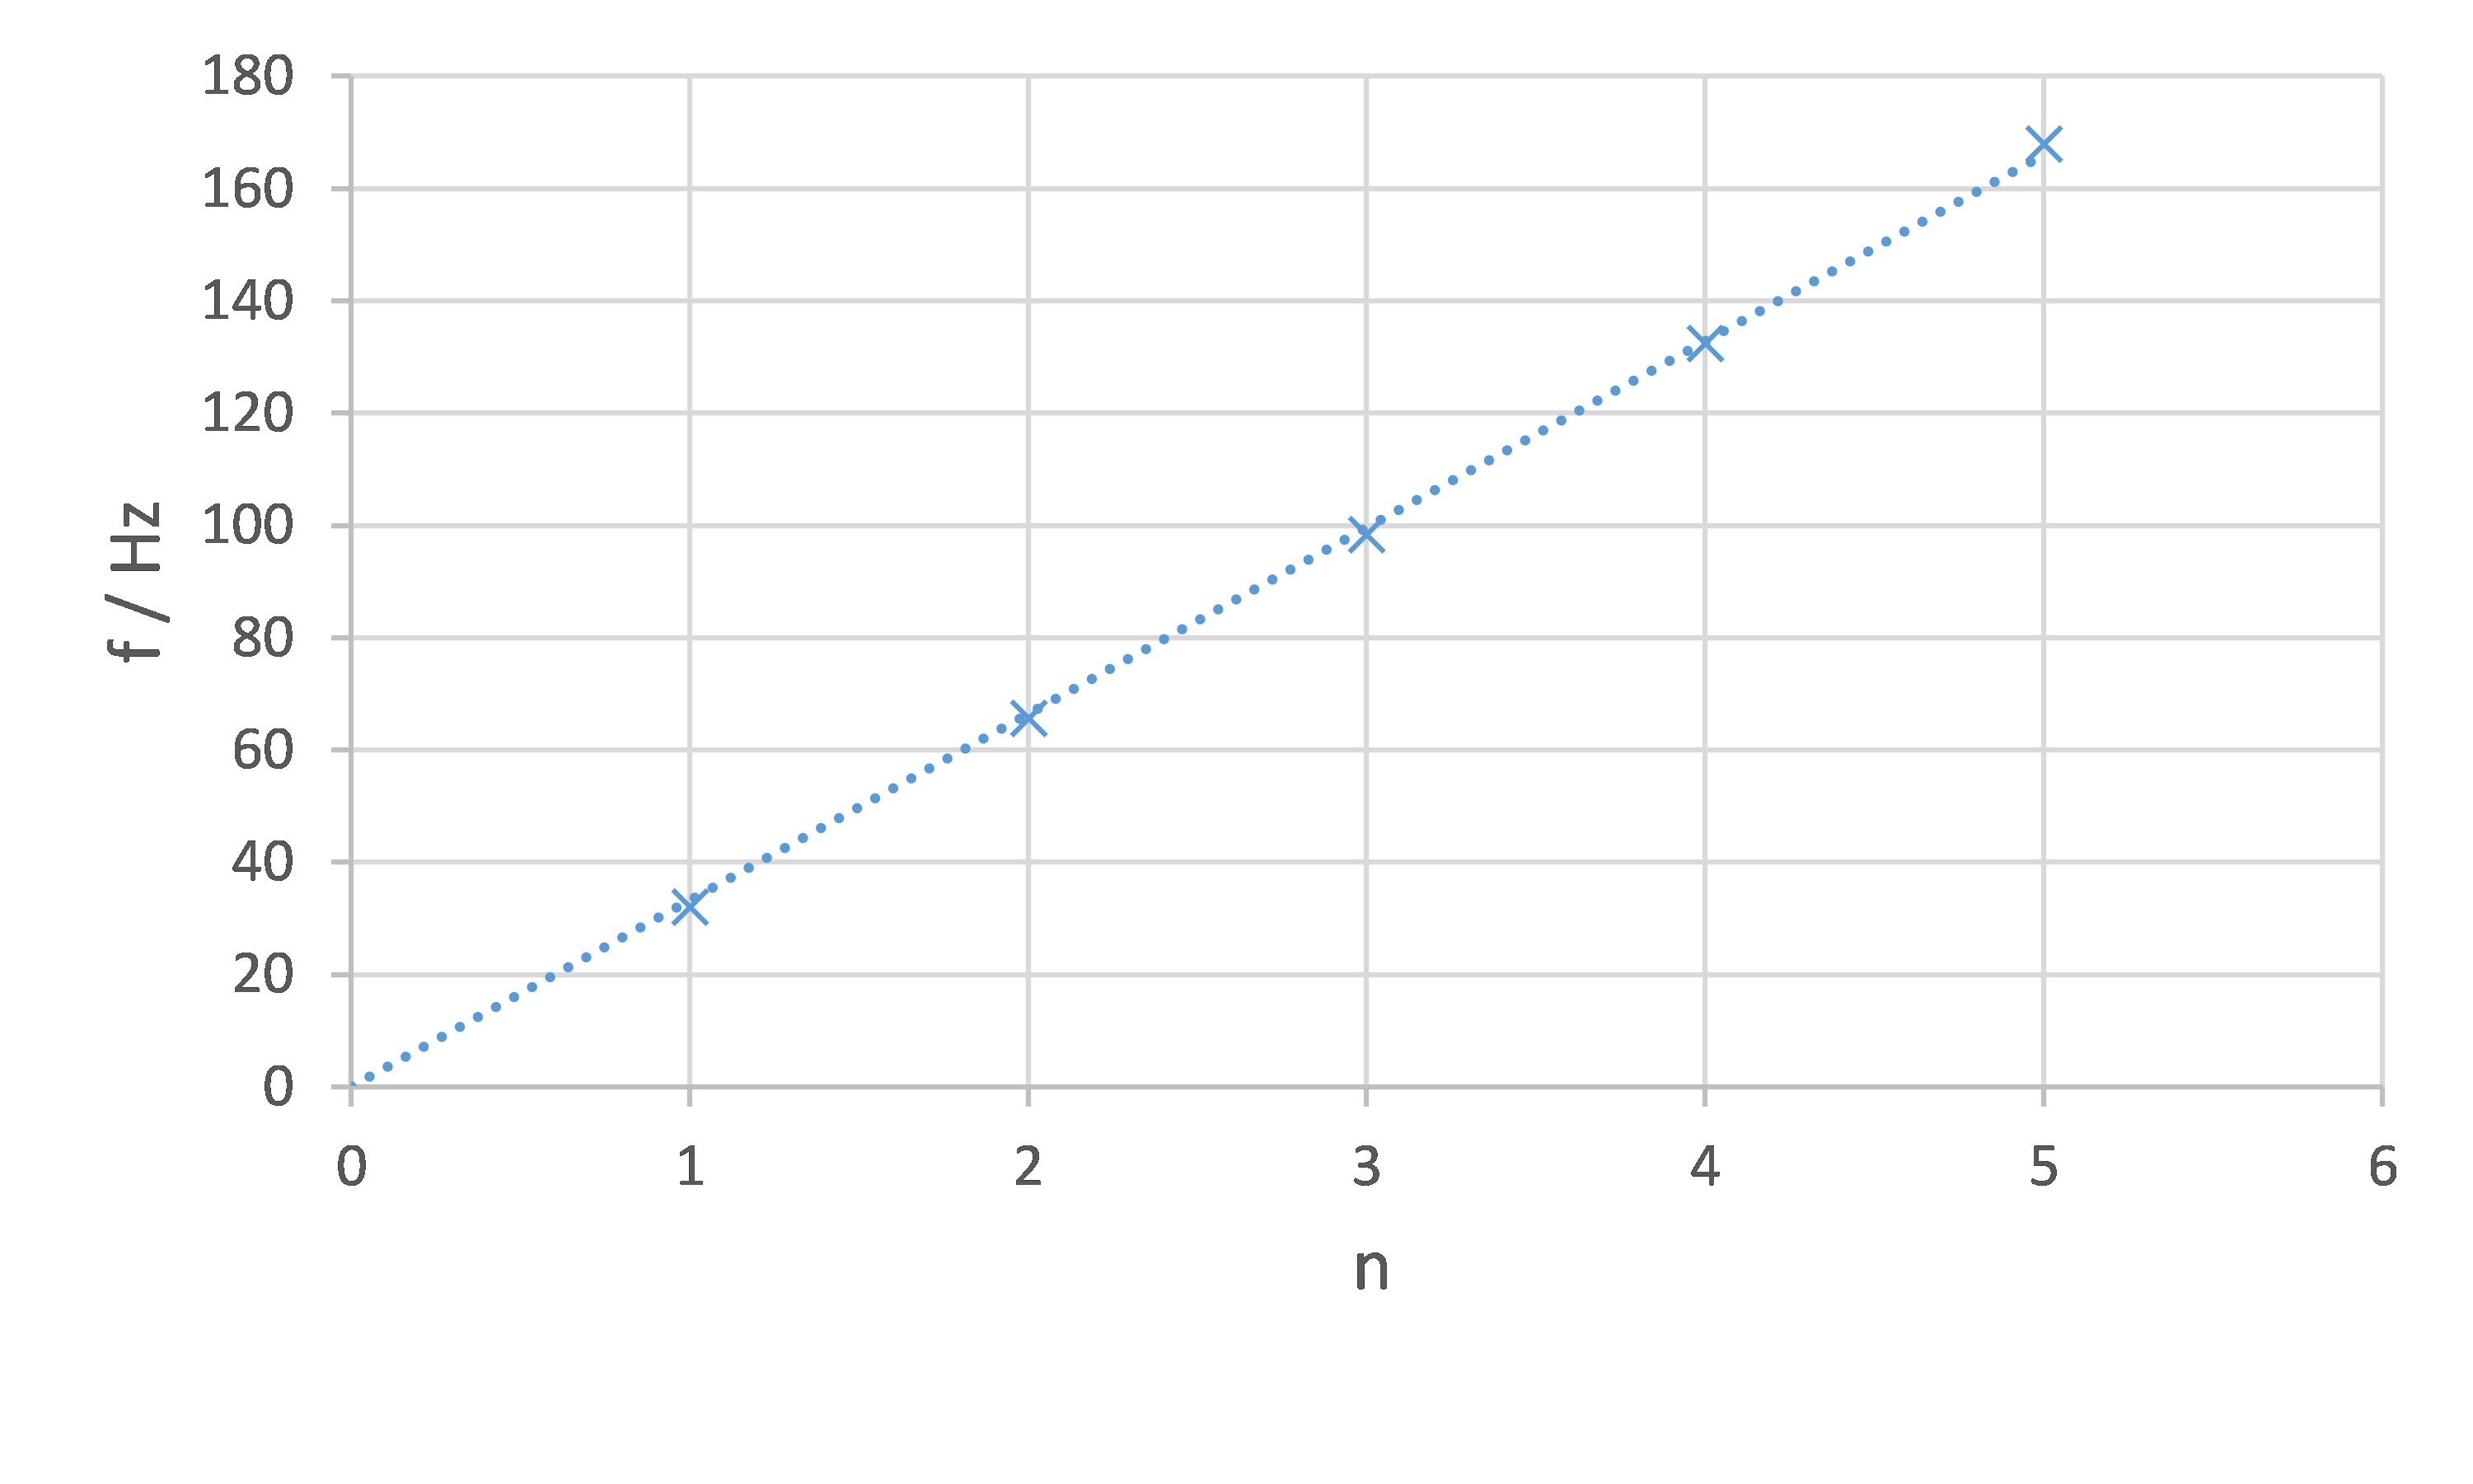
\includegraphics[scale=0.15]{1.png}
\caption{6\#弦线$f$与$n$关系图}}
\end{figure}
拟合直线斜率的相对不确定度$\frac{k}{U_k} = 2\%$,表明f与n的线性关系较好. 已知6\#弦线线密度为0.00936$kg/m$,则计算出理论斜率数值为$k_0=32.4Hz$,可见实验得出的斜率值与理论数值也比较接近.

\paragraph{对于5\#弦线的数据分析如下:}
\begin{center}
{\kaishu 表2\quad5\#弦线共振频率$f$与半波数$n$关系实验数据}
\begin{tabular}{|c|c|c|c|c|c|}
\hline
	{半波数\tiny\quad\normalsize$n$}&1&2&3&4&5\\
\hline
	{共振频率$f/Hz$}&{40.93}&{83.86}&{126.48}&{169.03}&{212.57}\\
\hline
\end{tabular}
\end{center}
\par 对5\#弦线半波数$n = 1 - 5$时共振频率$f$进行测量,所得数据如表2所示. 对此组数据利用Excel程序的linest函数对$f$和$n$做截距为0的最小二乘法直线拟合,设直线斜率为$k$,利用Excel程序的tinv函数计算$p = 0.95$时的$t$因子,可得到:\par
\begin{center}\begin{tabular}{r l}
{斜率}& {$k=42.31018Hz$}\\
{斜率标准偏差}& {$s_k=0.130889Hz$}\\
{t因子}& {$t_{0.95,4}=2.776445$}\\
{斜率不确定度}& {$U_k=t_{0.95,4}\times s_k = 0.363405Hz$}
\end{tabular}\end{center}
因此,f、n拟合得出的直线斜率为$k=(42.31\pm0.36)Hz$\par
\begin{figure}[H]\centering\kaishu{
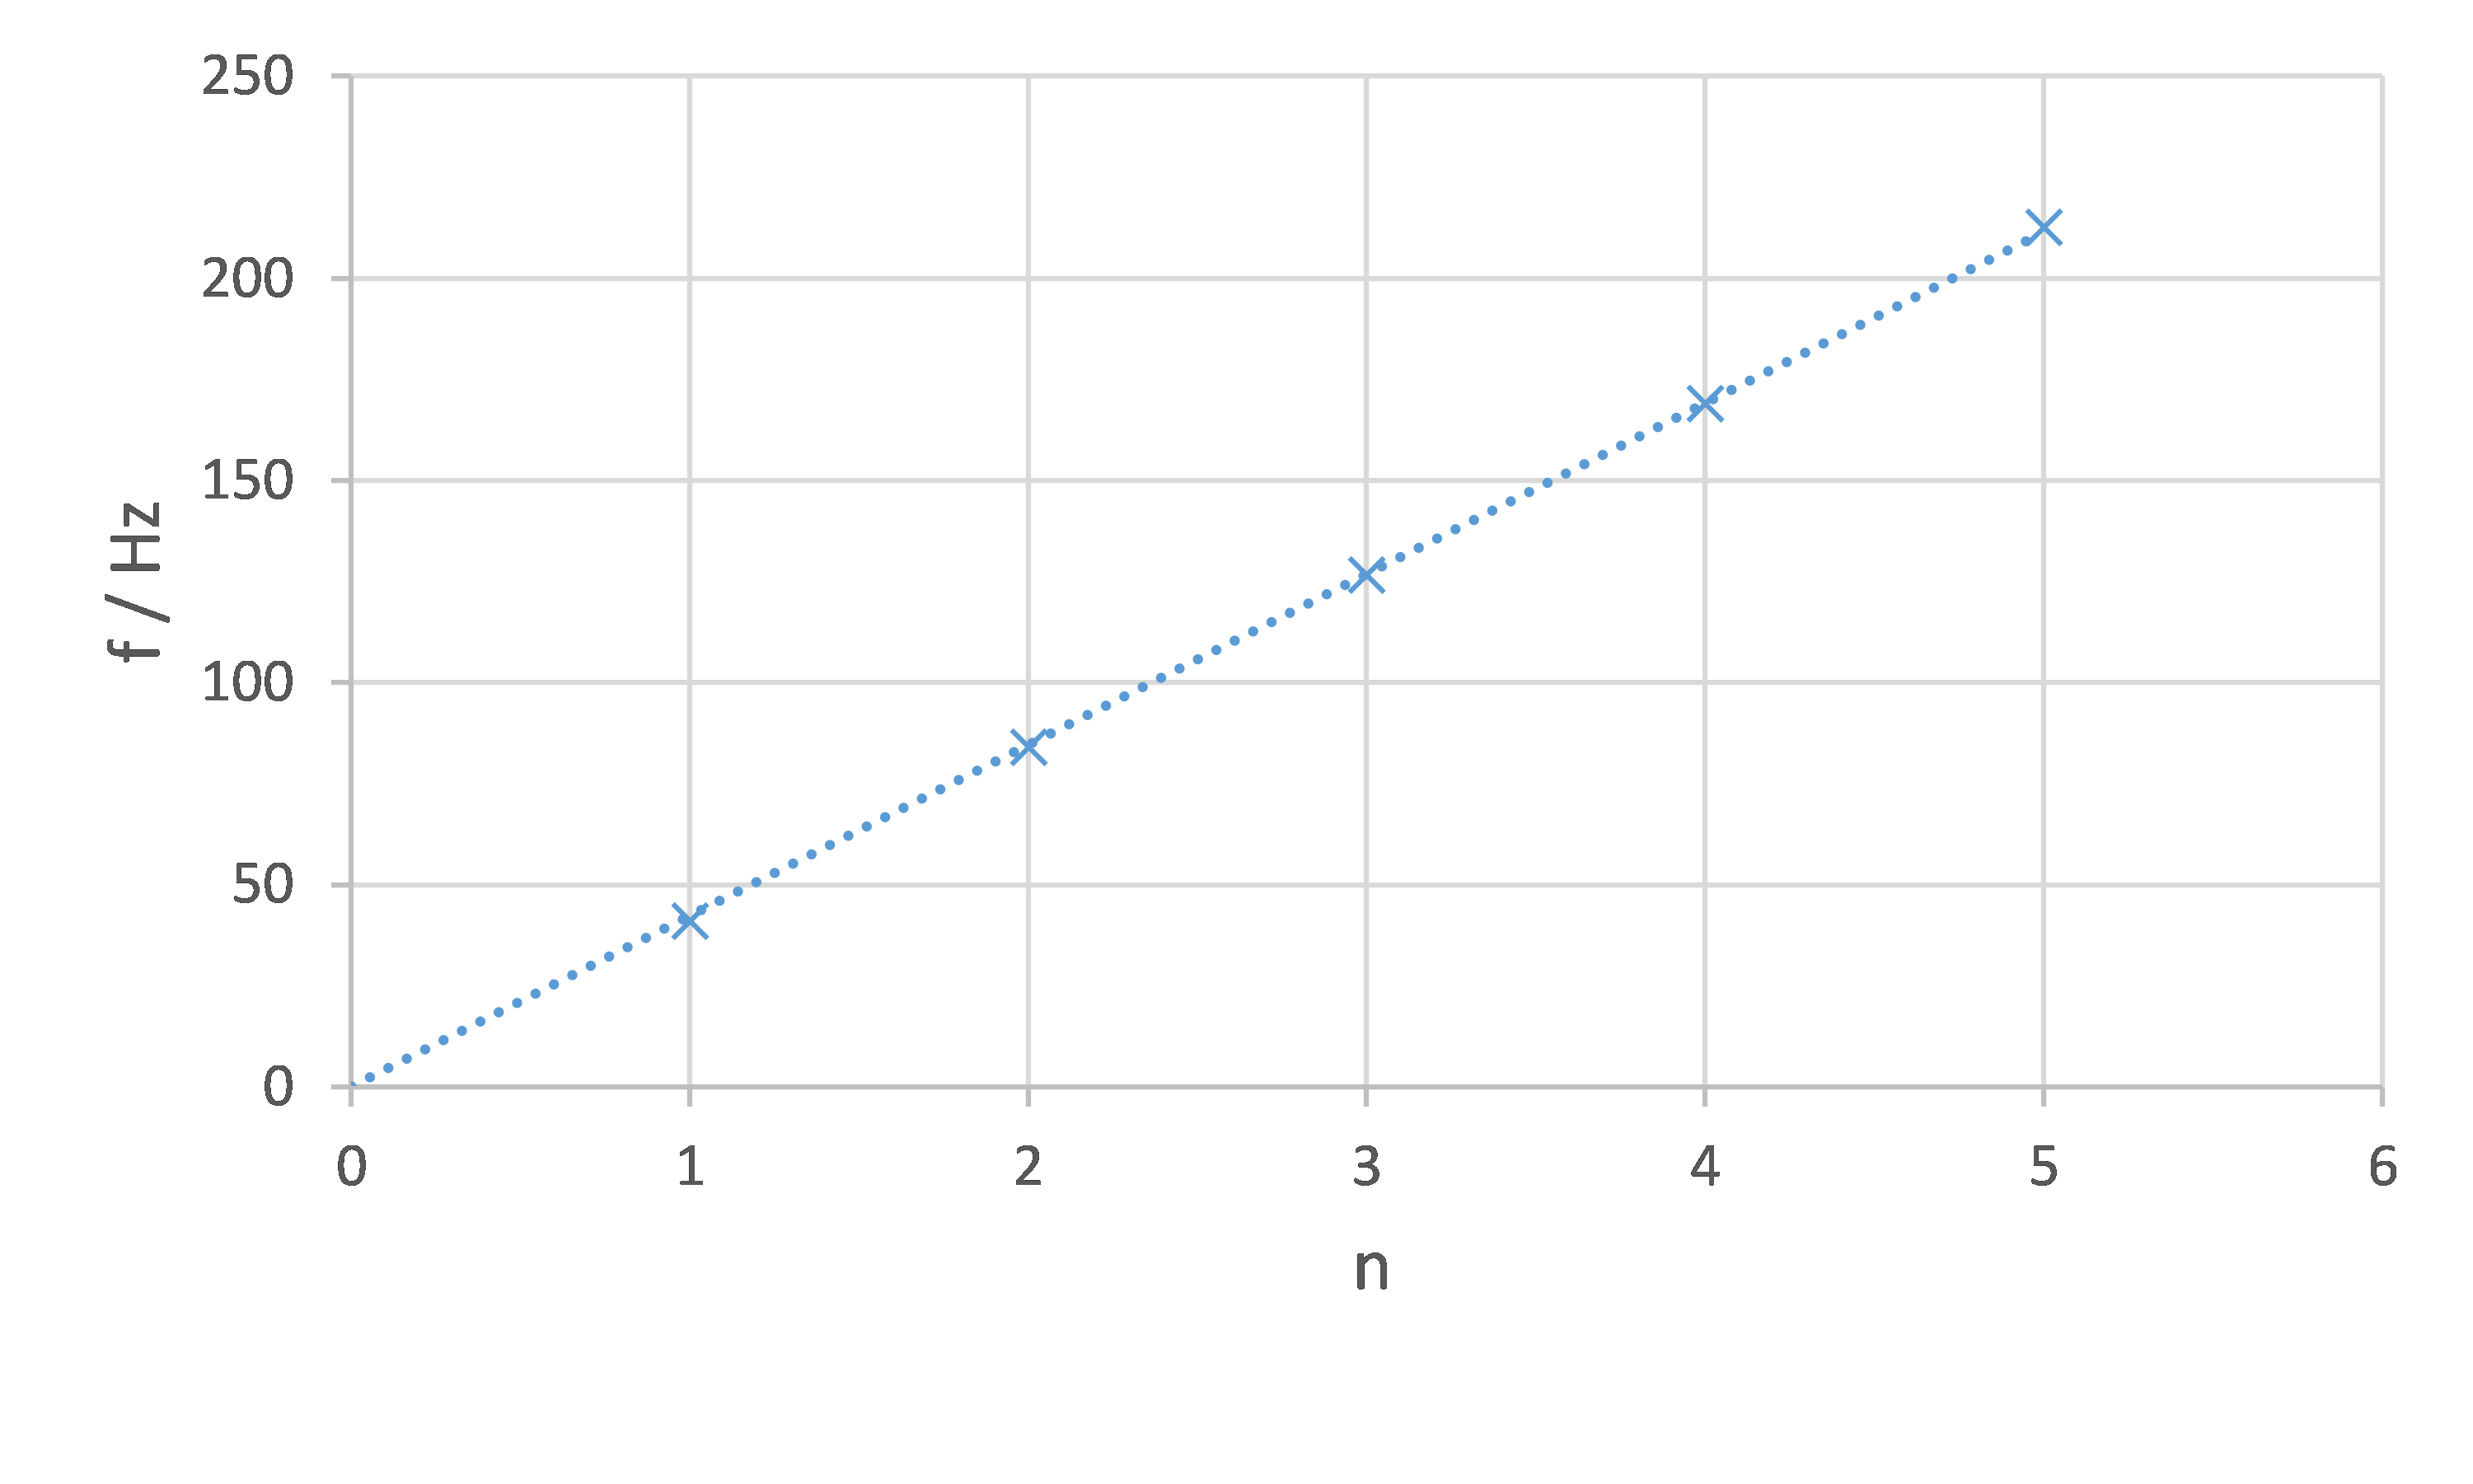
\includegraphics[scale=0.15]{2.png}
\caption{5\#弦线$f$与$n$关系图}}
\end{figure}
拟合直线斜率的相对不确定度$\frac{k}{U_k} = 0.8\%$,表明f与n的线性关系较好. 已知5\#弦线线密度为0.00578$kg/m$,则计算出理论斜率数值为$k_0=41.18Hz$,可见实验得出的斜率值与理论数值也比较接近.

\subsubsection*{B) 探究$f$与$L$的关系图}
采用控制变量法,需要控制$n$、$T$、$\rho$的数值. 在砝码钩上放置4个砝码,使得弦上张力为$F = 9.800N$. 调整信号发生器$V_pp = 5.000V$,用正弦波对弦进行激励,改变两个弦码之间的距离,在弦长$L = 30.00cm--55.00cm$六种情况下较粗的4\#和3\#弦线形成半波数$n = 1$的驻波时的共振频率进行测量.\par
由公式${f = \frac{n}{2L}\sqrt{\frac{T}{\rho}}}$计算对$f$与$\frac{1}{L}$拟合的截距为0的直线理论斜率$k_0$,直线斜率应为$k_0=\frac{n}{2}\sqrt{\frac{T}{\rho}}$.



\paragraph{对于4\#弦线的数据分析如下:}
\begin{center}
{\kaishu 表3\quad4\#弦线共振频率$f$与弦长倒数$\frac{1}{L}$关系实验数据}
\begin{tabular}{|c|c|c|c|c|c|c|}
\hline
	$L/cm$&55.00&50.00&45.00&40.00&35.00&30.00\\
\hline
	$\frac{1}{L}/m^{-1}$&1.818&2.000&2.222&2.500&2.857&3.333\\
\hline
	{$f/Hz$}&{47.17}&{52.61}&{57.22}&{64.92}&{74.67}&{87.75}\\
\hline
\end{tabular}
\end{center}
\par 对4\#弦长${L} = 30.00cm - 55.00cm$时共振频率$f$进行测量,所得数据如表3所示. 对此组数据利用Excel程序的linest函数对$\frac{1}{L}$和$f$做截距为0的最小二乘法直线拟合,设直线斜率为$k$,利用Excel程序的tinv函数计算$p = 0.95$时的$t$因子,可得到:\par
\begin{center}\begin{tabular}{r l}
{斜率}& {$k=26.11555Hz\cdot m$}\\
{斜率标准偏差}& {$s_k=0.090065Hz\cdot m$}\\
{t因子}& {$t_{0.95,5}=2.570582$}\\
{斜率不确定度}& {$U_k=t_{0.95,5}\times s_k = 0.231519Hz\cdot m$}
\end{tabular}\end{center}
因此,f、$\frac{1}{L}$拟合得出的直线斜率为$k=(26.11\pm0.23)Hz\cdot m$\par
\begin{figure}[H]\centering\kaishu{
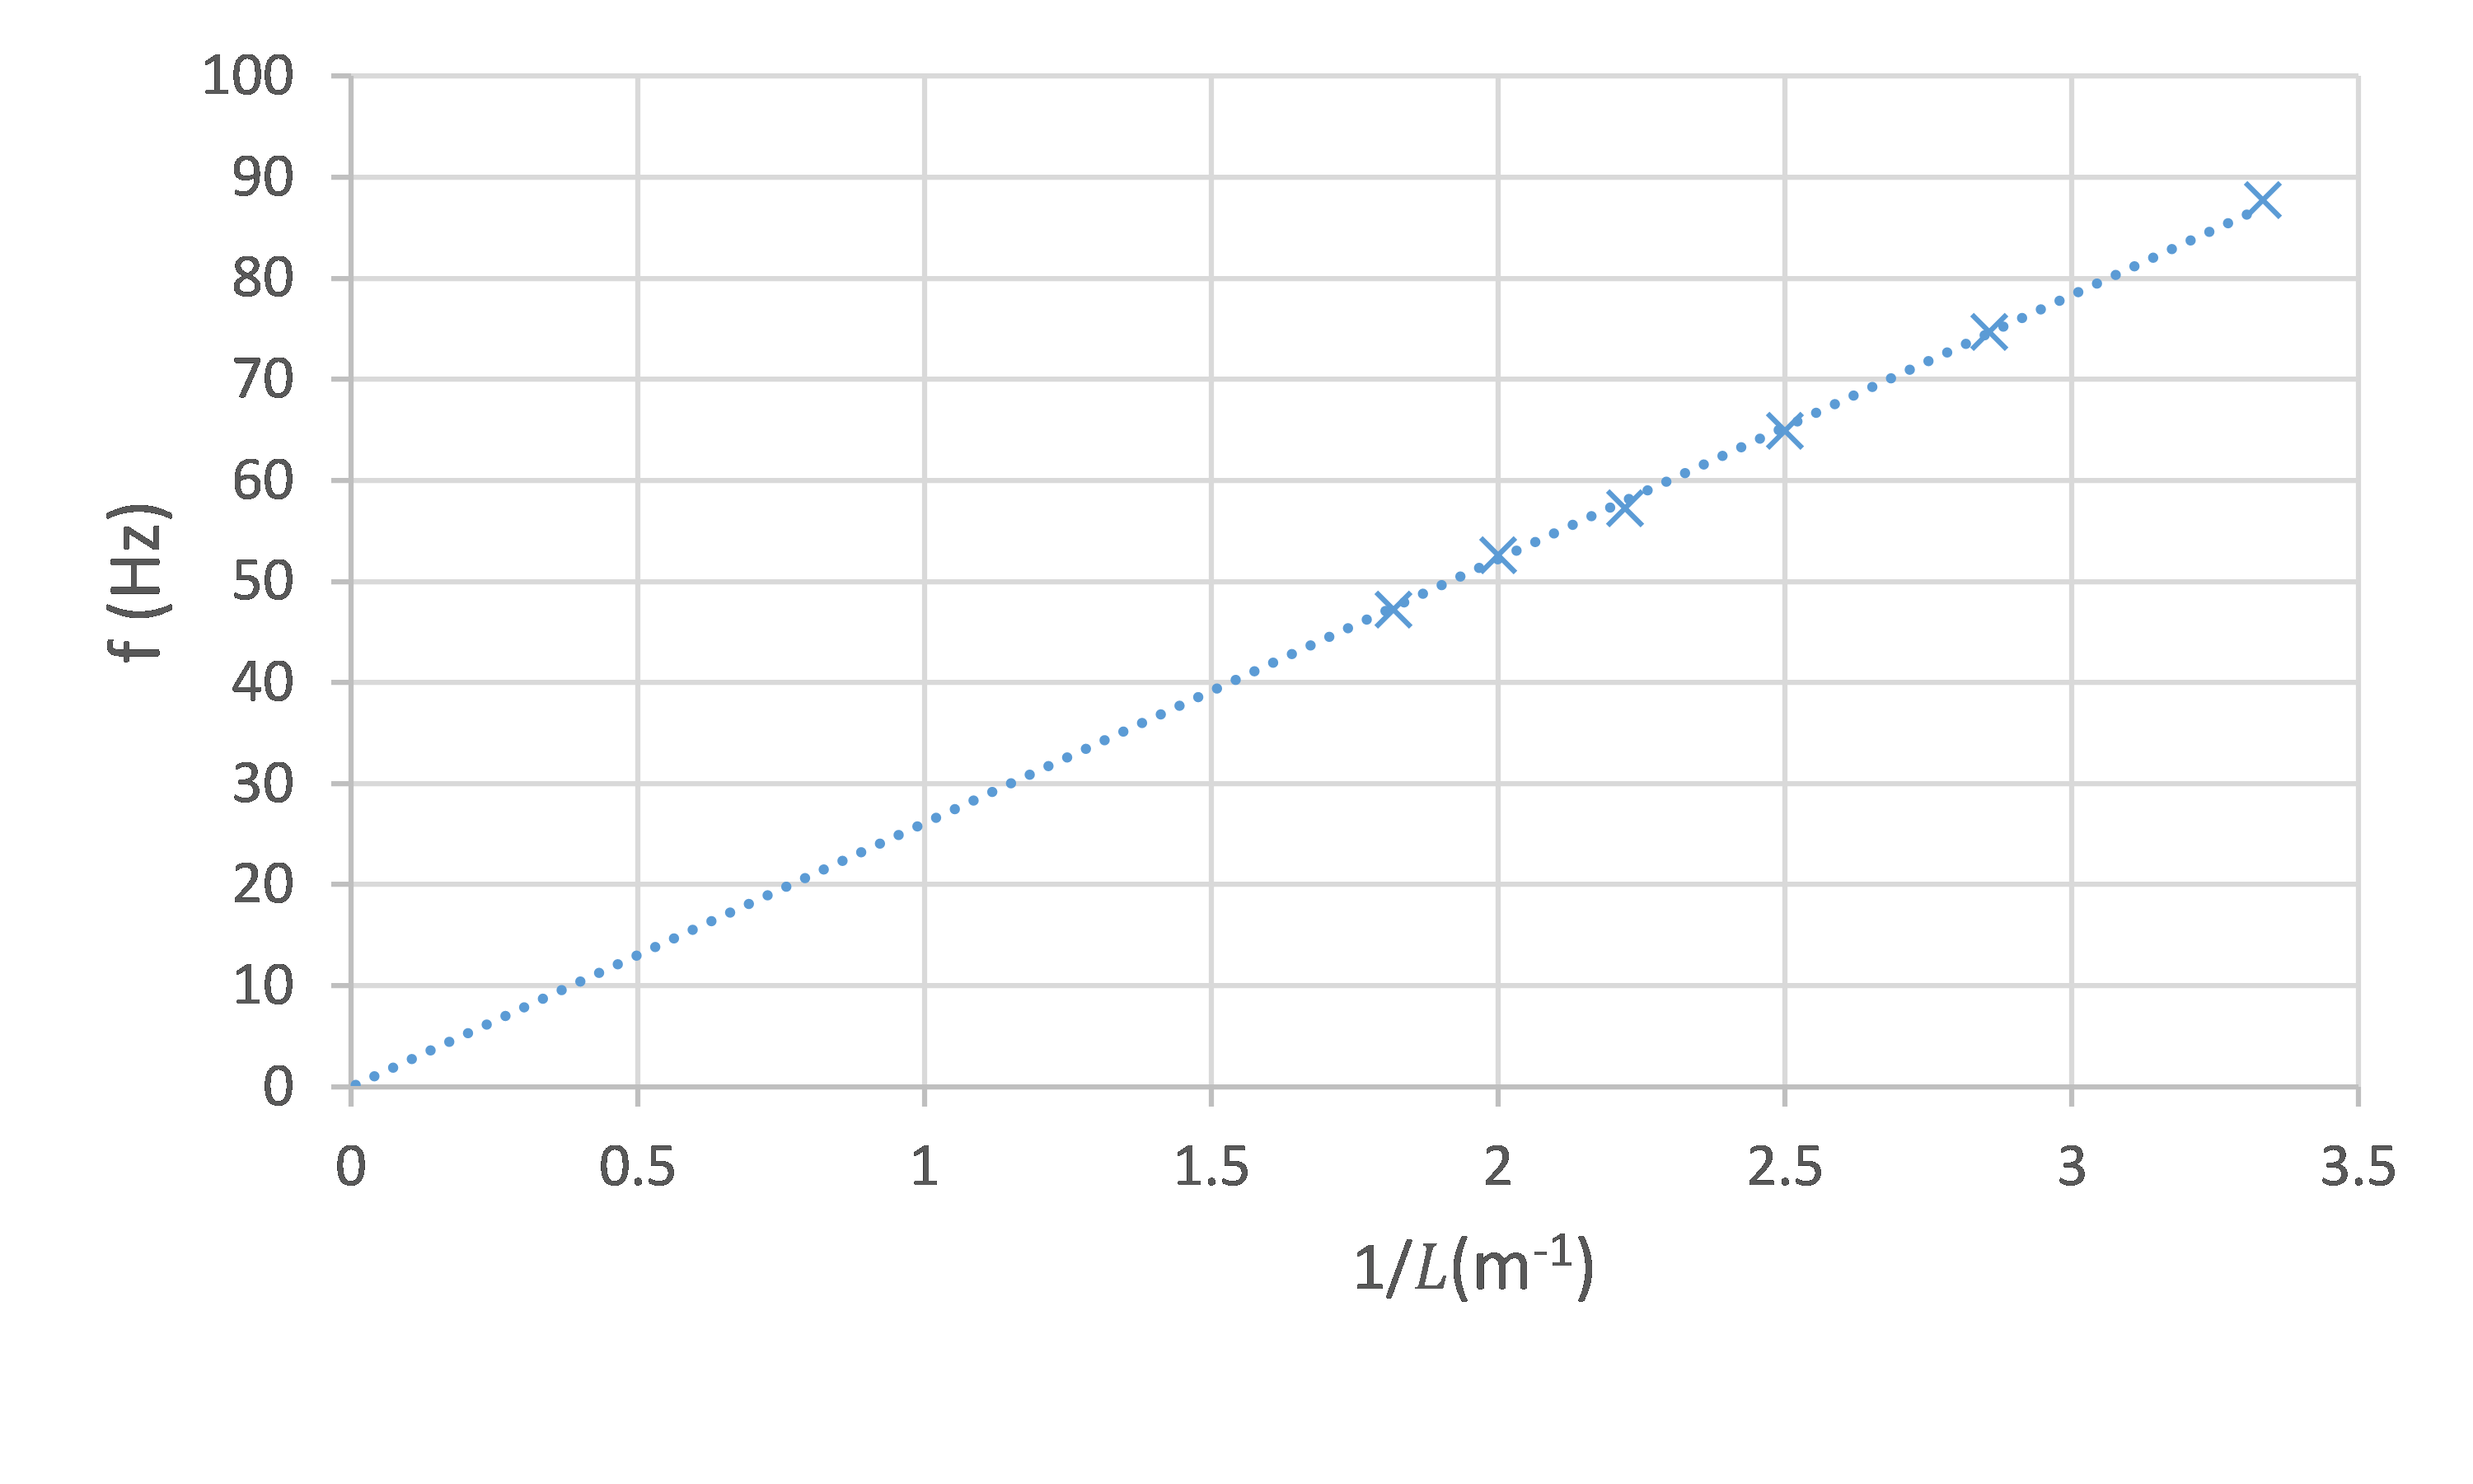
\includegraphics[scale=0.15]{3.png}
\caption{4\#弦线$f$与$\frac{1}{L}$关系图}}
\end{figure}
拟合直线斜率的相对不确定度$\frac{k}{U_k} = 0.9\%$,表明f与n的线性关系较好. 已知4\#弦线线密度为0.00350$kg/m$,则计算出理论斜率数值为$k_0=26.46Hz\cdot m$,可见实验得出的斜率值与理论数值也比较接近.

\paragraph{对于3\#弦线的数据分析如下:}
\begin{center}
{\kaishu 表4\quad3\#弦线共振频率$f$与弦长倒数$\frac{1}{L}$关系实验数据}
\begin{tabular}{|c|c|c|c|c|c|c|}
\hline
	$L/cm$&55.00&50.00&45.00&40.00&35.00&30.00\\
\hline
	$\frac{1}{L}/m^{-1}$&1.818&2.000&2.222&2.500&2.857&3.333\\
\hline
	{$f/Hz$}&{63.87}&{69.28}&{78.35}&{88.39}&{101.17}&{117.40}\\
\hline
\end{tabular}
\end{center}
\par 对3\#弦长${L} = 30.00cm - 55.00cm$时共振频率$f$进行测量,所得数据如表3所示. 对此组数据利用Excel程序的linest函数对$\frac{1}{L}$和$f$做截距为0的最小二乘法直线拟合,设直线斜率为$k$,利用Excel程序的tinv函数计算$p = 0.95$时的$t$因子,可得到:\par
\begin{center}\begin{tabular}{r l}
{斜率}& {$k=35.22112Hz\cdot m$}\\
{斜率标准偏差}& {$s_k=0.097469Hz\cdot m$}\\
{t因子}& {$t_{0.95,5}=2.570582$}\\
{斜率不确定度}& {$U_k=t_{0.95,5}\times s_k = 0.250551Hz\cdot m$}
\end{tabular}\end{center}
因此,f、$\frac{1}{L}$拟合得出的直线斜率为$k=(35.22\pm0.25)Hz\cdot m$\par
\begin{figure}[H]\centering\kaishu{
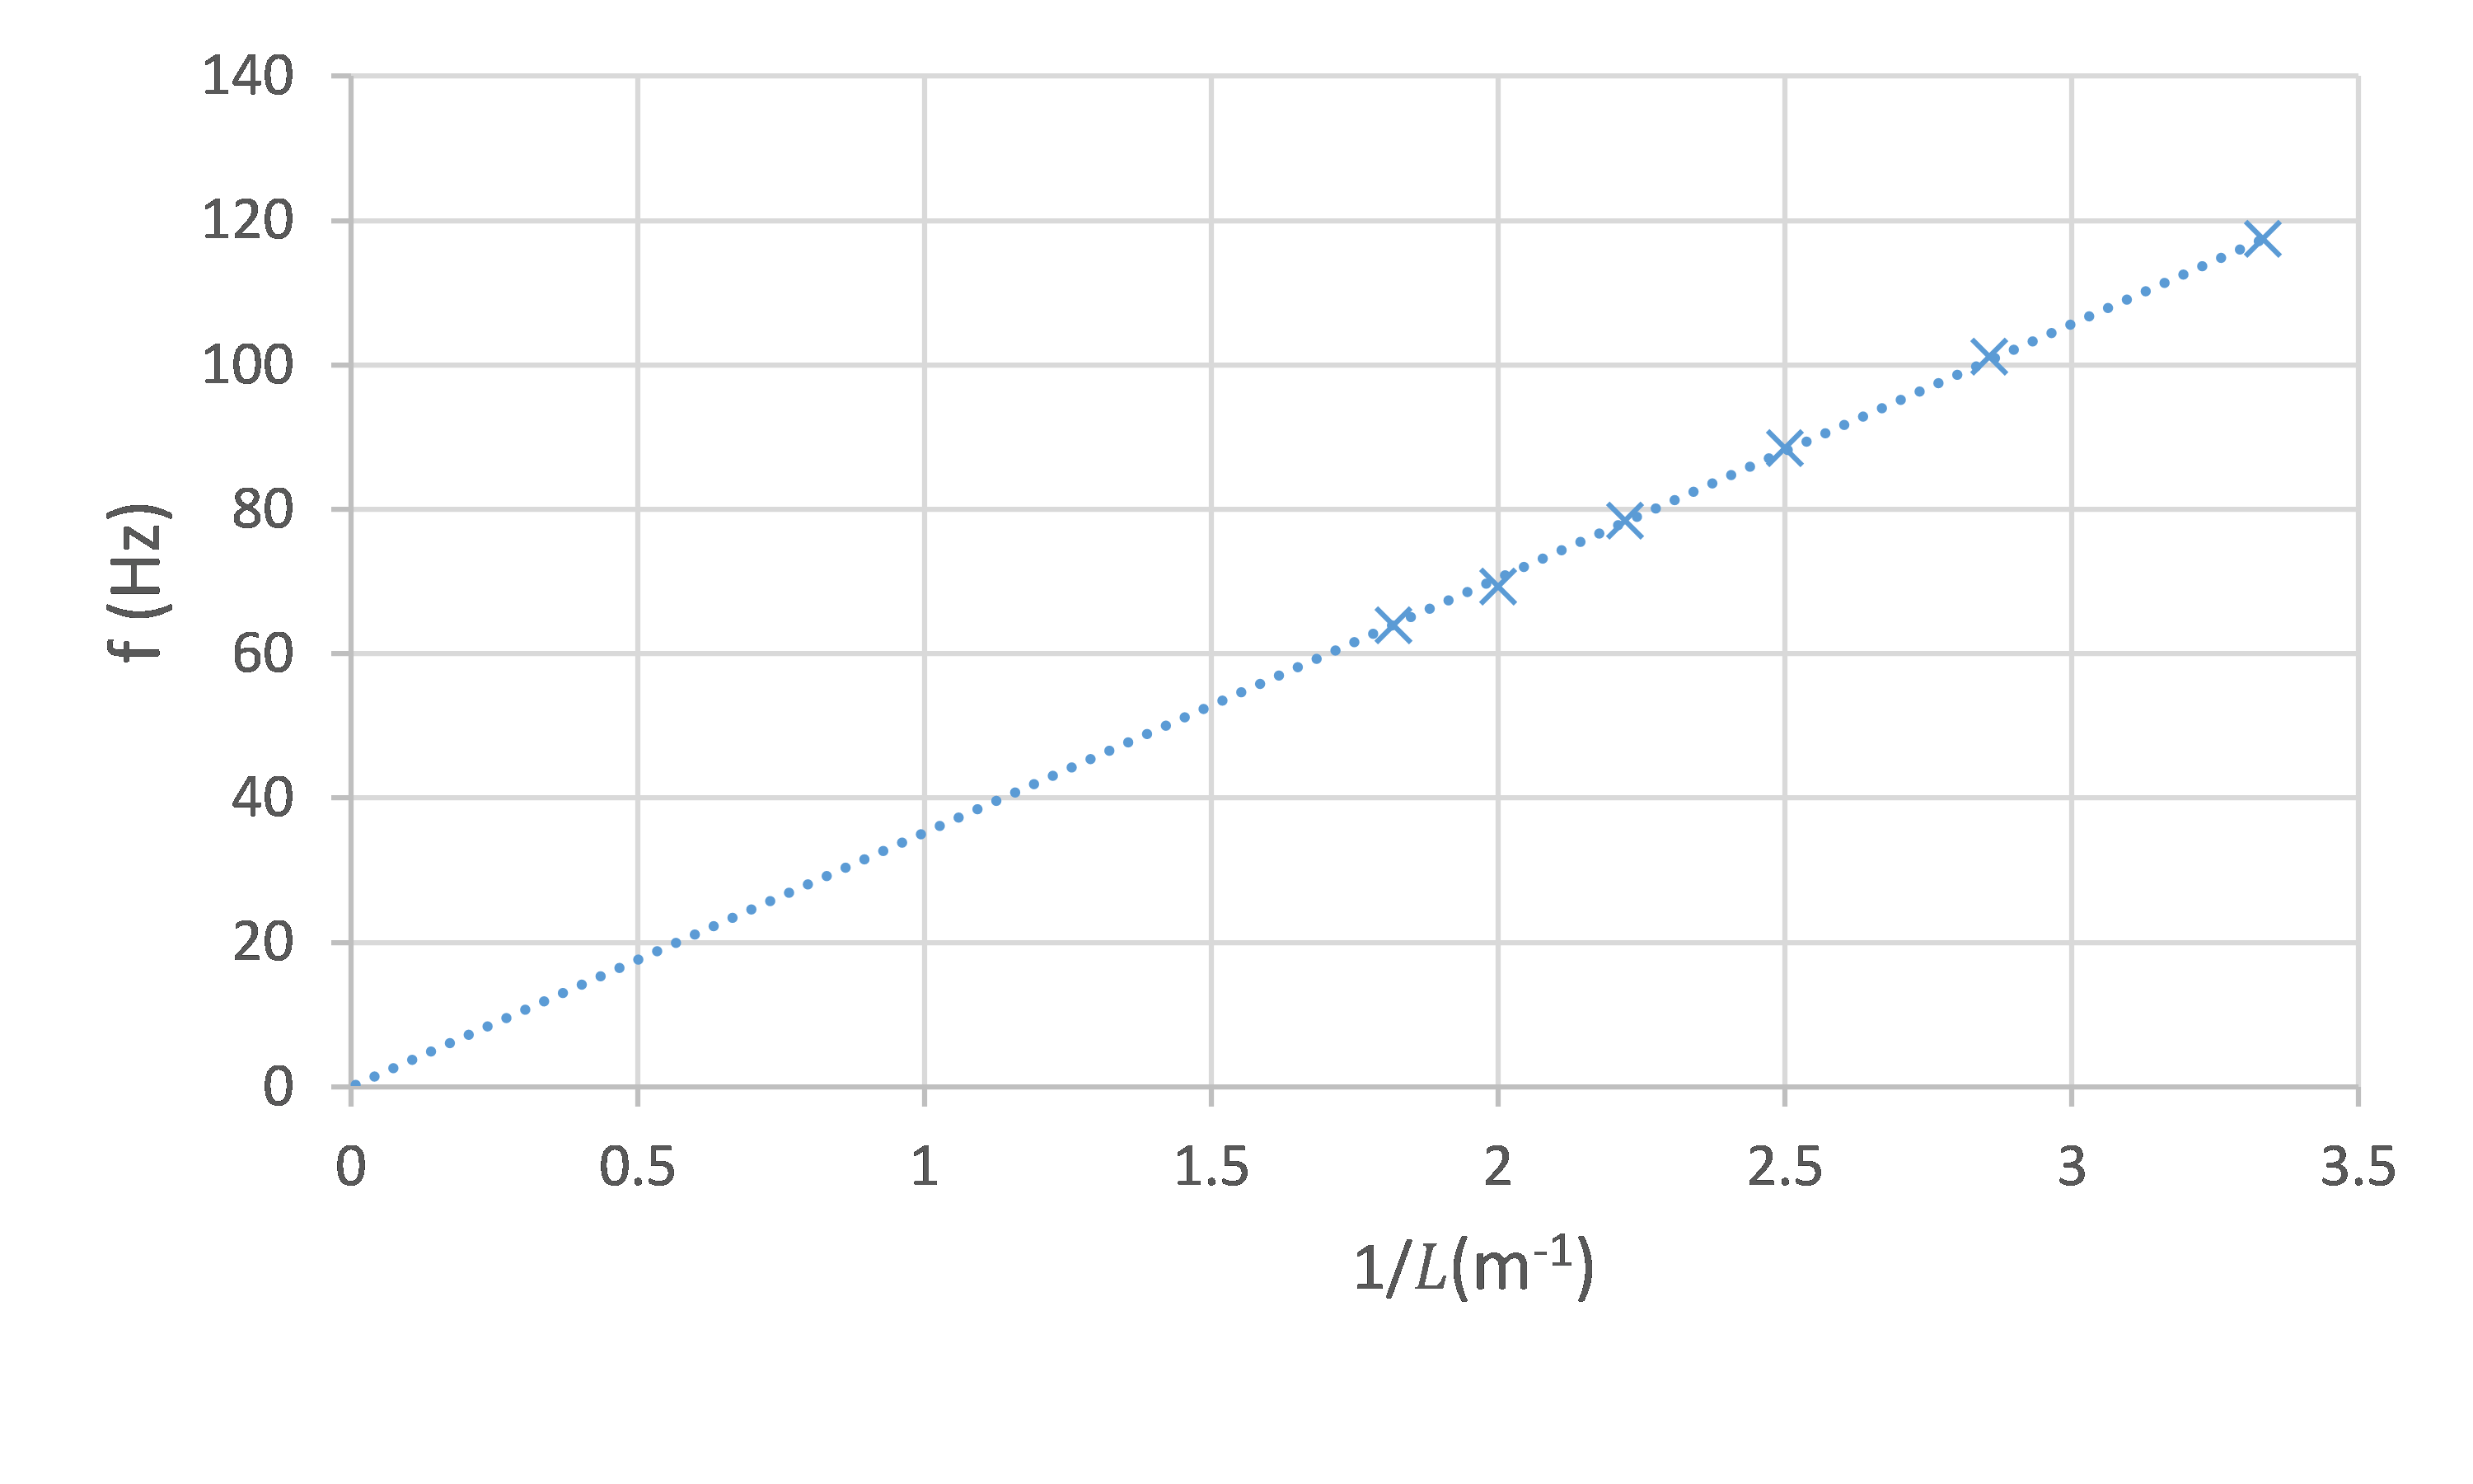
\includegraphics[scale=0.15]{4.png}
\caption{3\#弦线$ln(f)$与$ln(T)$关系图}}
\end{figure}
拟合直线斜率的相对不确定度$\frac{k}{U_k} = 0.7\%$,表明f与n的线性关系较好. 已知3\#弦线线密度为0.00191$kg/m$,则计算出理论斜率数值为$k_0=35.81Hz\cdot m$,可见实验得出的斜率值与理论数值也比较接近.


\subsubsection*{C) 探究$f$与$T$的关系}
采用控制变量法,需要控制$n$、$L$、$\rho$的数值. 调整两个弦码之间的距离,保持弦长$L = 50.00cm$,调整信号发生器$V_{pp} = 5.000V$,用正弦波对弦进行激励,改变砝码钩($200g$)上的砝码数量(每个$200g$),在砝码钩上砝码为0 - 5个(分别对应弦上张力$T=1.960N, 3.920N, 5.880N, 7.840N, 9.800N, 11.760N$)六种情况下较细的2\#和1\#弦线形成半波数$n = 1$的驻波时的共振频率进行测量.\par
由公式${f = \frac{n}{2L}\sqrt{\frac{T}{\rho}}}$,可得等式$ln(f)=ln(n)-ln(2L)+\frac{1}{2}T-\frac{1}{2}\rho$. 设$ln(f)$与$ln(T)$直线拟合的理论斜率$k_0$,截距$b_0$,直线斜率应为$k_0=0.500$,$b_0=ln(n)-ln(2L)-\frac{1}{2}ln(\rho)$.

\paragraph{对于2\#弦线的数据分析如下:}
\begin{center}
{\kaishu 表5\quad2\#弦线共振频率$ln(f)$与弦上张力$ln(T)$关系实验数据}
\begin{tabular}{|c|c|c|c|c|c|c|}
\hline
	$T/N$&1.960&3.920&5.880&7.840&9.800&11.760\\
\hline
	$ln(T)$&0.6729&1.366&1.772&2.059&2.282&2.465\\
\hline
	$f/Hz$&43.24&59.67&74.57&87.17&97.01&105.67\\
\hline
	$ln(f)$&3.767&4.089&4.312&4.468&4.575&4.660\\
\hline
\end{tabular}
\end{center}
\par 对2\#弦上张力=${T} = 1.960N - 11.760N$时共振频率$f$进行测量,所得数据如表所示. 对此组数据利用Excel程序的linest函数对$ln(f)$和$ln(T)$最小二乘法直线拟合,设直线斜率为$k$,截距为$b$,利用Excel程序的tinv函数计算$p = 0.95$时的$t$因子,可得到:\par
\begin{center}\begin{tabular}{r l}
{斜率}& {$k=0.505558$}\\
{斜率标准偏差}& {$s_k=0.00805$}\\
{截距}&{$b=3.4171$}\\
{截距标准偏差}&{$s_b=0.01505$}\\
{t因子}& {$t_{0.95,5}=2.776445$}\\
{斜率不确定度}& {$U_k=t_{0.95,5}\times s_k = 0.02234$}\\
{截距不确定度}& {$U_b=t_{0.95,5}\times s_b = 0.04177$}
\end{tabular}\end{center}
因此,$ln(f)$、$ln(T)$拟合得出的直线斜率为$k=(0.506\pm0.022)$,截距为$b=(3.417\pm0.042).$\par
\begin{figure}[H]\centering\kaishu{
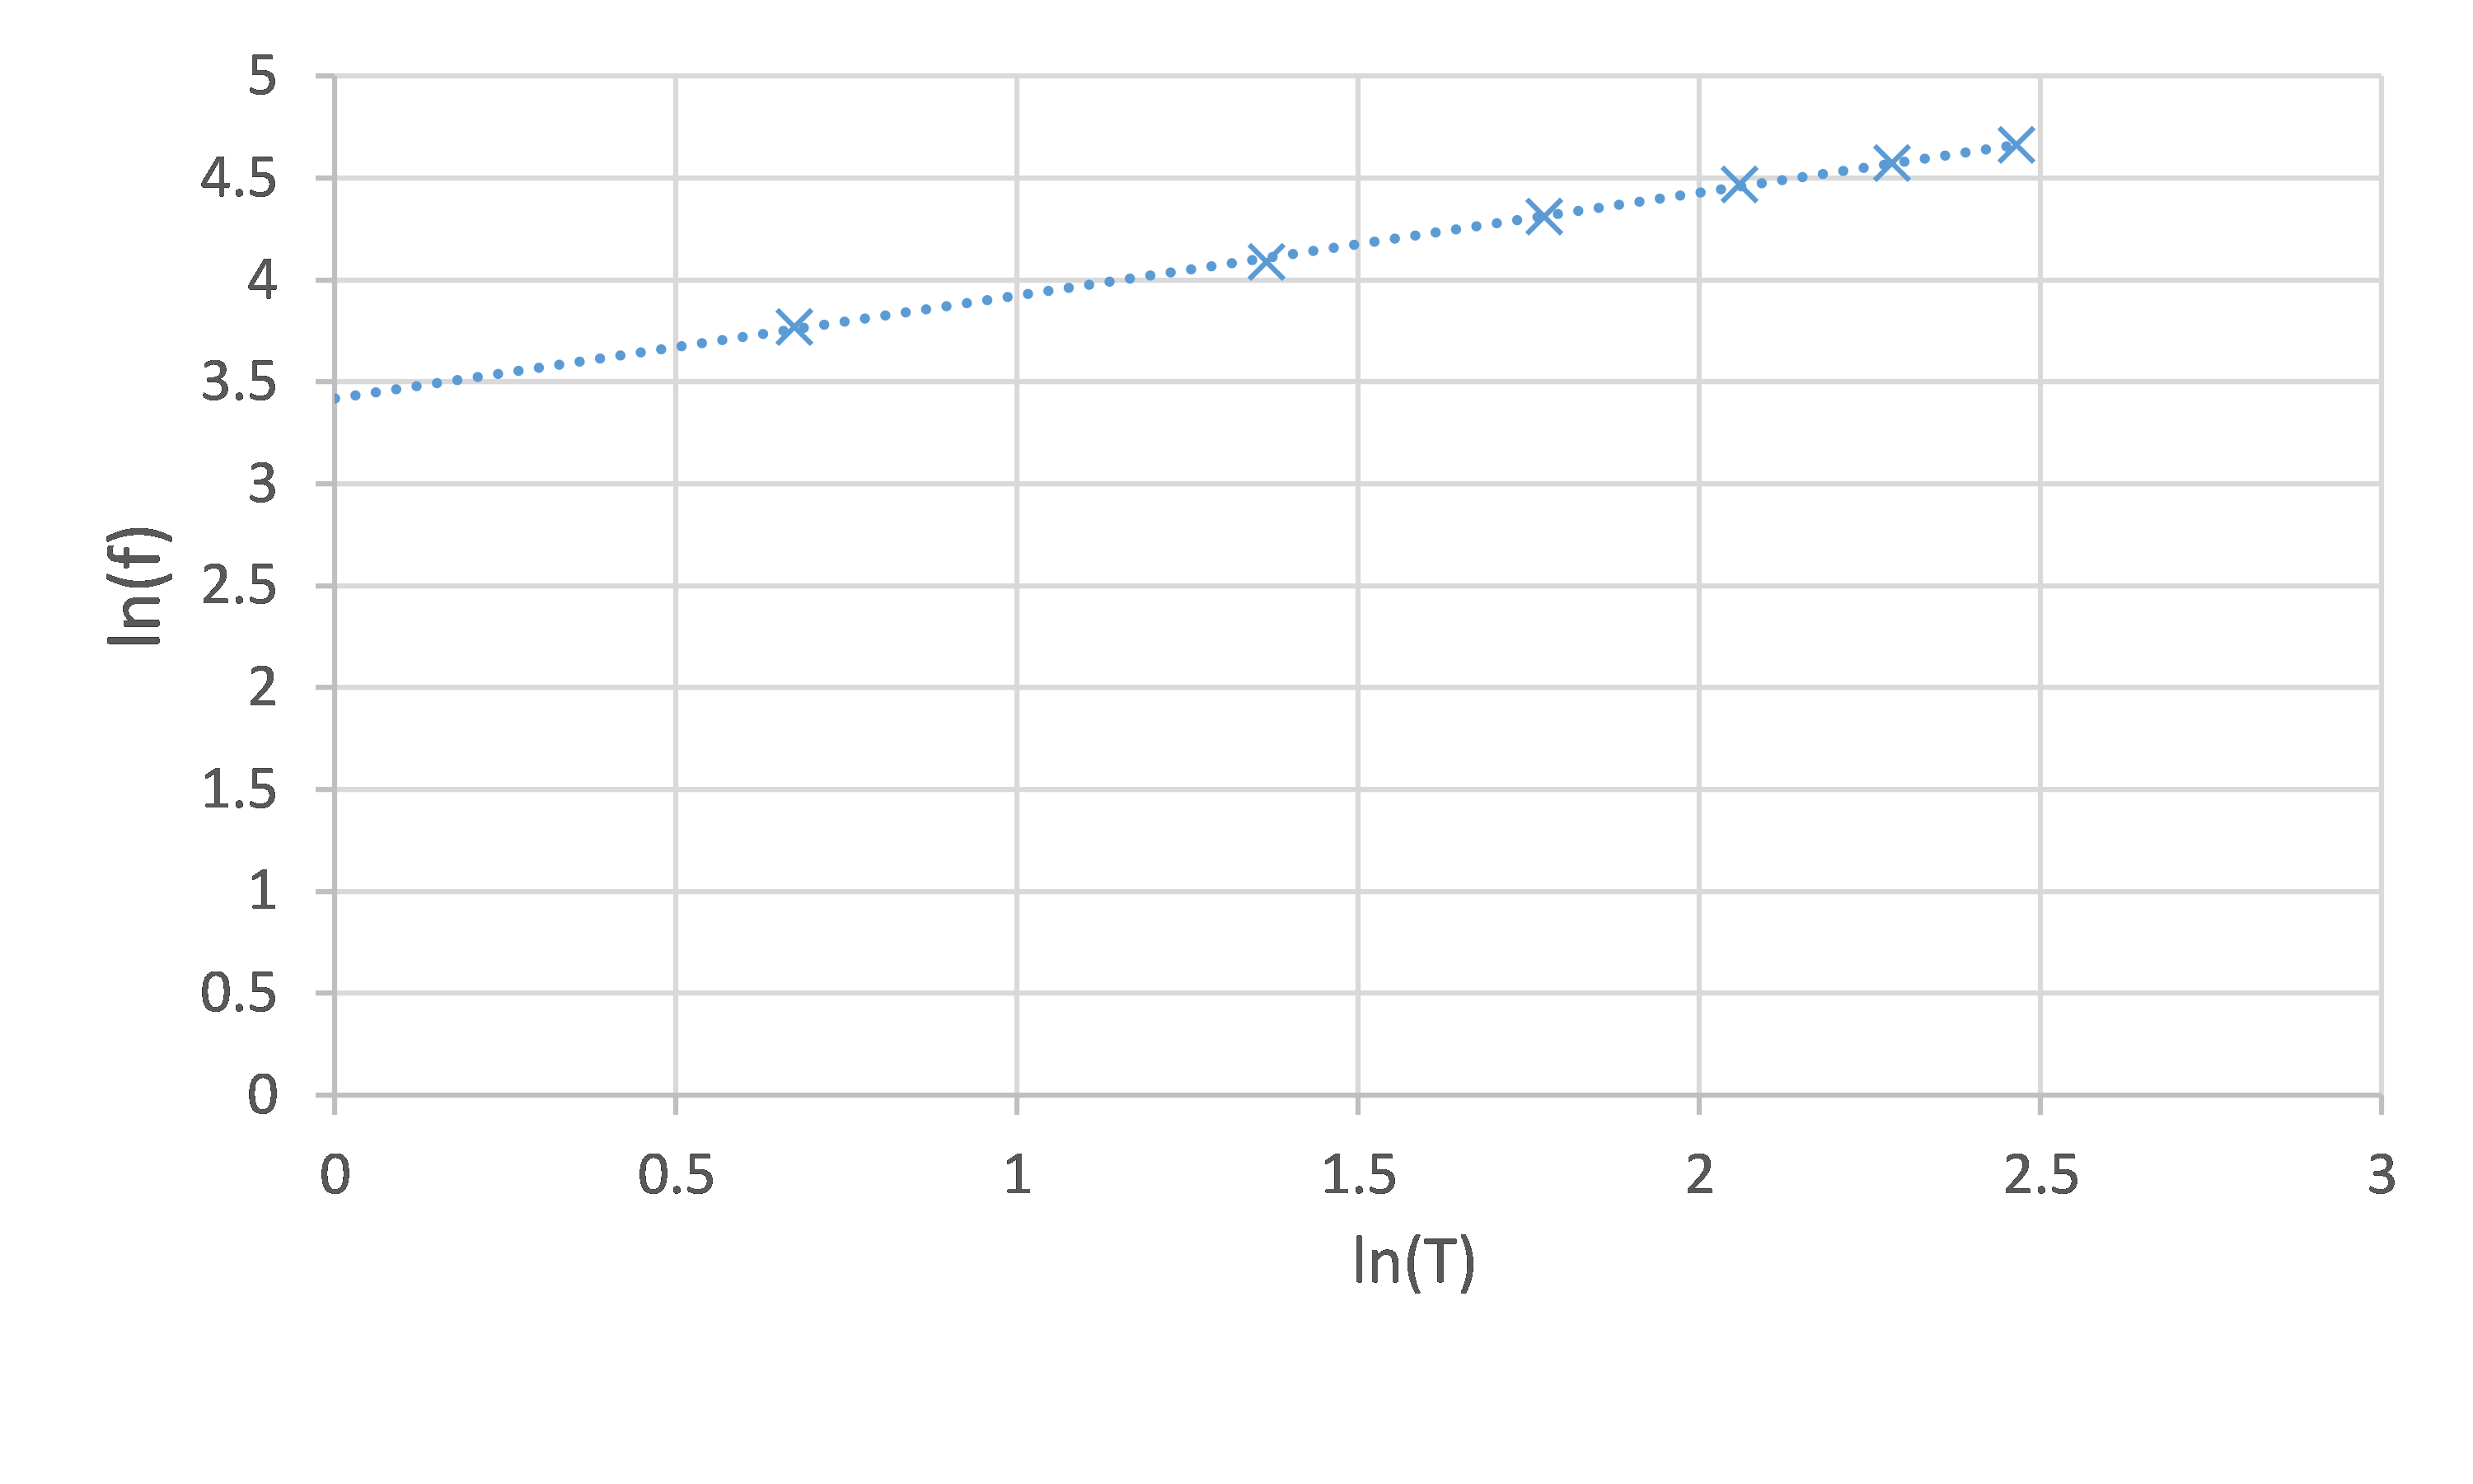
\includegraphics[scale=0.15]{5.png}
\caption{2\#弦线$ln(f)$与$ln(T)$关系图}}
\end{figure}
拟合直线斜率的相对不确定度$\frac{k}{U_k} = 4\%$,截距的相对不确定度$\frac{b}{U_b} = 1\%$,表明f与n的线性关系较好. 4\#弦线线密度为$0.00191kg/m$,计算理论斜率与截距,直线斜率理论值应为$k_0=0.500$,截距应为$b_0=3.464$,可见实验得出的斜率和截距与理论数值也比较接近.

\paragraph{对于1\#弦线的数据分析如下:}
\begin{center}
{\kaishu 表6\quad1\#弦线共振频率$ln(f)$与弦上张力$ln(T)$关系实验数据}
\begin{tabular}{|c|c|c|c|c|c|c|}
\hline
	$T/N$&1.960&3.920&5.880&7.840&9.800&11.760\\
\hline
	$ln(T)$&0.6729&1.366&1.772&2.059&2.282&2.465\\
\hline
	$f/Hz$&57.51&81.65&99.77&115.56&129.47&140.91\\
\hline
	$ln(f)$&4.012&4.402&4.603&4.750&4.863&4.948\\
\hline
\end{tabular}
\end{center}
\par 对1\#弦上张力=${T} = 1.960N - 11.760N$时共振频率$f$进行测量,所得数据如表所示. 对此组数据利用Excel程序的linest函数对$ln(f)$和$ln(T)$最小二乘法直线拟合,设直线斜率为$k$,截距为$b$,利用Excel程序的tinv函数计算$p = 0.95$时的$t$因子,可得到:\par
\begin{center}\begin{tabular}{r l}
{斜率}& {$k=0.50157$}\\
{斜率标准偏差}& {$s_k=0.00197$}\\
{截距}&{$b=3.71559$}\\
{截距标准偏差}&{$s_b=0.00368$}\\
{t因子}& {$t_{0.95,5}=2.776445$}\\
{斜率不确定度}& {$U_k=t_{0.95,5}\times s_k = 0.00547$}\\
{截距不确定度}& {$U_b=t_{0.95,5}\times s_b = 0.01023$}
\end{tabular}\end{center}
因此,$ln(f)$、$ln(T)$拟合得出的直线斜率为$k=(0.502\pm0.005)$,截距为$b=(3.716\pm0.010).$\par
\begin{figure}\centering\kaishu{
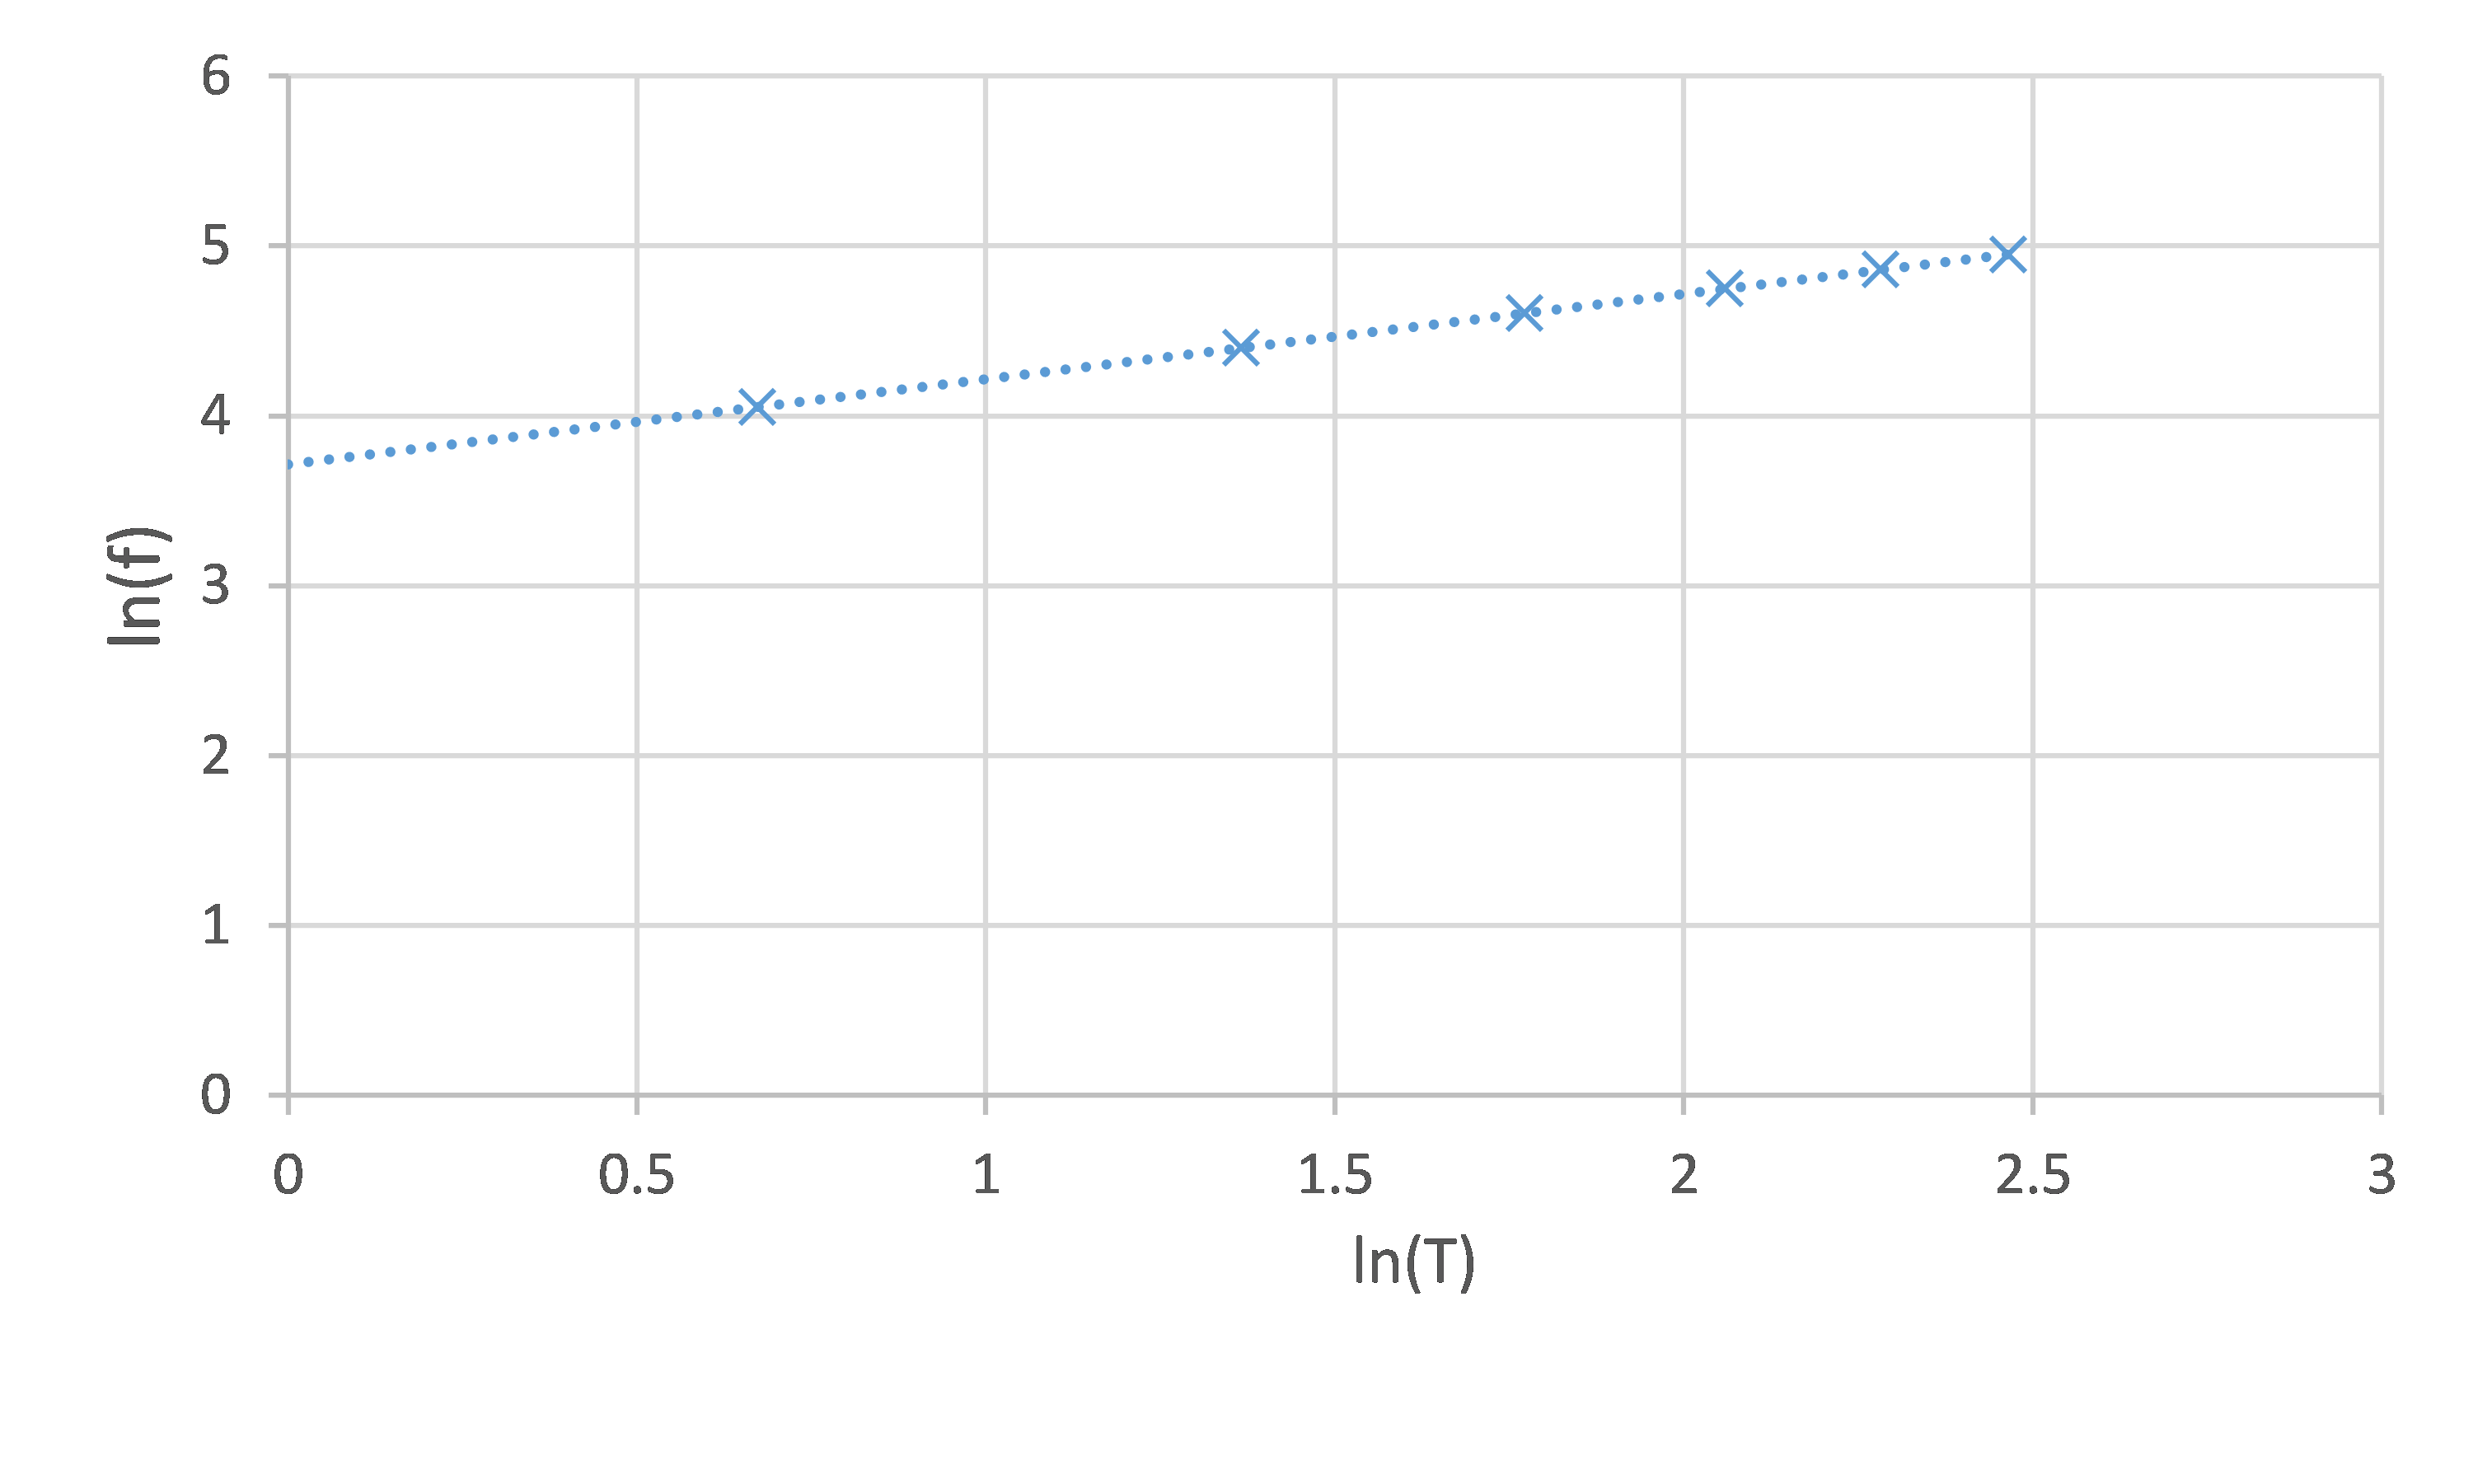
\includegraphics[scale=0.15]{6.png}
\caption{1\#弦线$ln(f)$与$ln(T)$关系图}}
\end{figure}
拟合直线斜率的相对不确定度$\frac{k}{U_k} = 1\%$,截距的相对不确定度$\frac{b}{U_b} = 0.2\%$,表明f与n的线性关系较好. 4\#弦线线密度为$0.00055kg/m$,计算理论斜率与截距,直线斜率应为$k_0=0.500$,截距应为$b_0=3.753$,可见实验得出的斜率和截距与理论数值也比较接近.


\subsubsection*{D) 探究$f$与$\rho$的关系}
此组实验数据可采用前述A)、B)、C)获得的部分数据. 采用控制变量法,需要控制$n$、$L$、$T$的数值. 取已有实验条件为$n=1$、$L=50.00cm$、$T=9.800N$的实验数据,对1\# - 6\#六根弦线在$V_{pp}=5.000V$正弦激励下的基频频率进行分析. \par
由公式${f = \frac{n}{2L}\sqrt{\frac{T}{\rho}}}$,可得等式$ln(f)=ln(n)-ln(2L)+\frac{1}{2}T-\frac{1}{2}\rho$. 设$ln(f)$与$ln(T)$直线拟合的理论斜率$k_0$,截距$b_0$,直线斜率应为$k_0=-0.500$,$b_0=ln(n)-ln(2L)+\frac{1}{2}ln(T)$.
\paragraph{数据分析如下:}
\begin{center}
{\kaishu 表7\quad1\# - 6\#弦线基频频率$ln(f)$与弦线密度$ln(\rho)$关系实验数据}
\begin{tabular}{|c|c|c|c|c|c|c|}
\hline
	$\rho/N$&0.00055&0.00098&0.00191&0.00350&0.00578&0.00936\\
\hline
	$ln(\rho)$&-7.506&-6.928&-6.261&-5.655&-5.153&-4.671\\
\hline
	$f/Hz$&129.47&97.01&69.28&52.61&40.93&31.91\\
\hline
	$ln(f)$&4.863&4.575&4.238&3.963&3.7119&3.4629\\
\hline
\end{tabular}
\end{center}
\par 对1\# - 6\#弦基频频率进行测量,所得数据如表7所示. 对此组数据利用Excel程序的linest函数对$ln(f)$和$ln(T)$最小二乘法直线拟合,设直线斜率为$k$,截距为$b$,利用Excel程序的tinv函数计算$p = 0.95$时的$t$因子,可得到:\par
\begin{center}\begin{tabular}{r l}
{斜率}& {$k=-0.4907$}\\
{斜率标准偏差}& {$s_k=0.00379$}\\
{截距}&{$b=1.17718$}\\
{截距标准偏差}&{$s_b=0.02314$}\\
{t因子}& {$t_{0.95,5}=2.776445$}\\
{斜率不确定度}& {$U_k=t_{0.95,5}\times s_k = 0.00974$}\\
{截距不确定度}& {$U_b=t_{0.95,5}\times s_b = 0.005947$}
\end{tabular}\end{center}
因此,$ln(f)$、$ln(\rho)$拟合得出的直线斜率为$k=(-0.491\pm0.010)$,截距为$b=(1.177\pm0.006).$\par
\begin{figure}[H]\centering\kaishu{
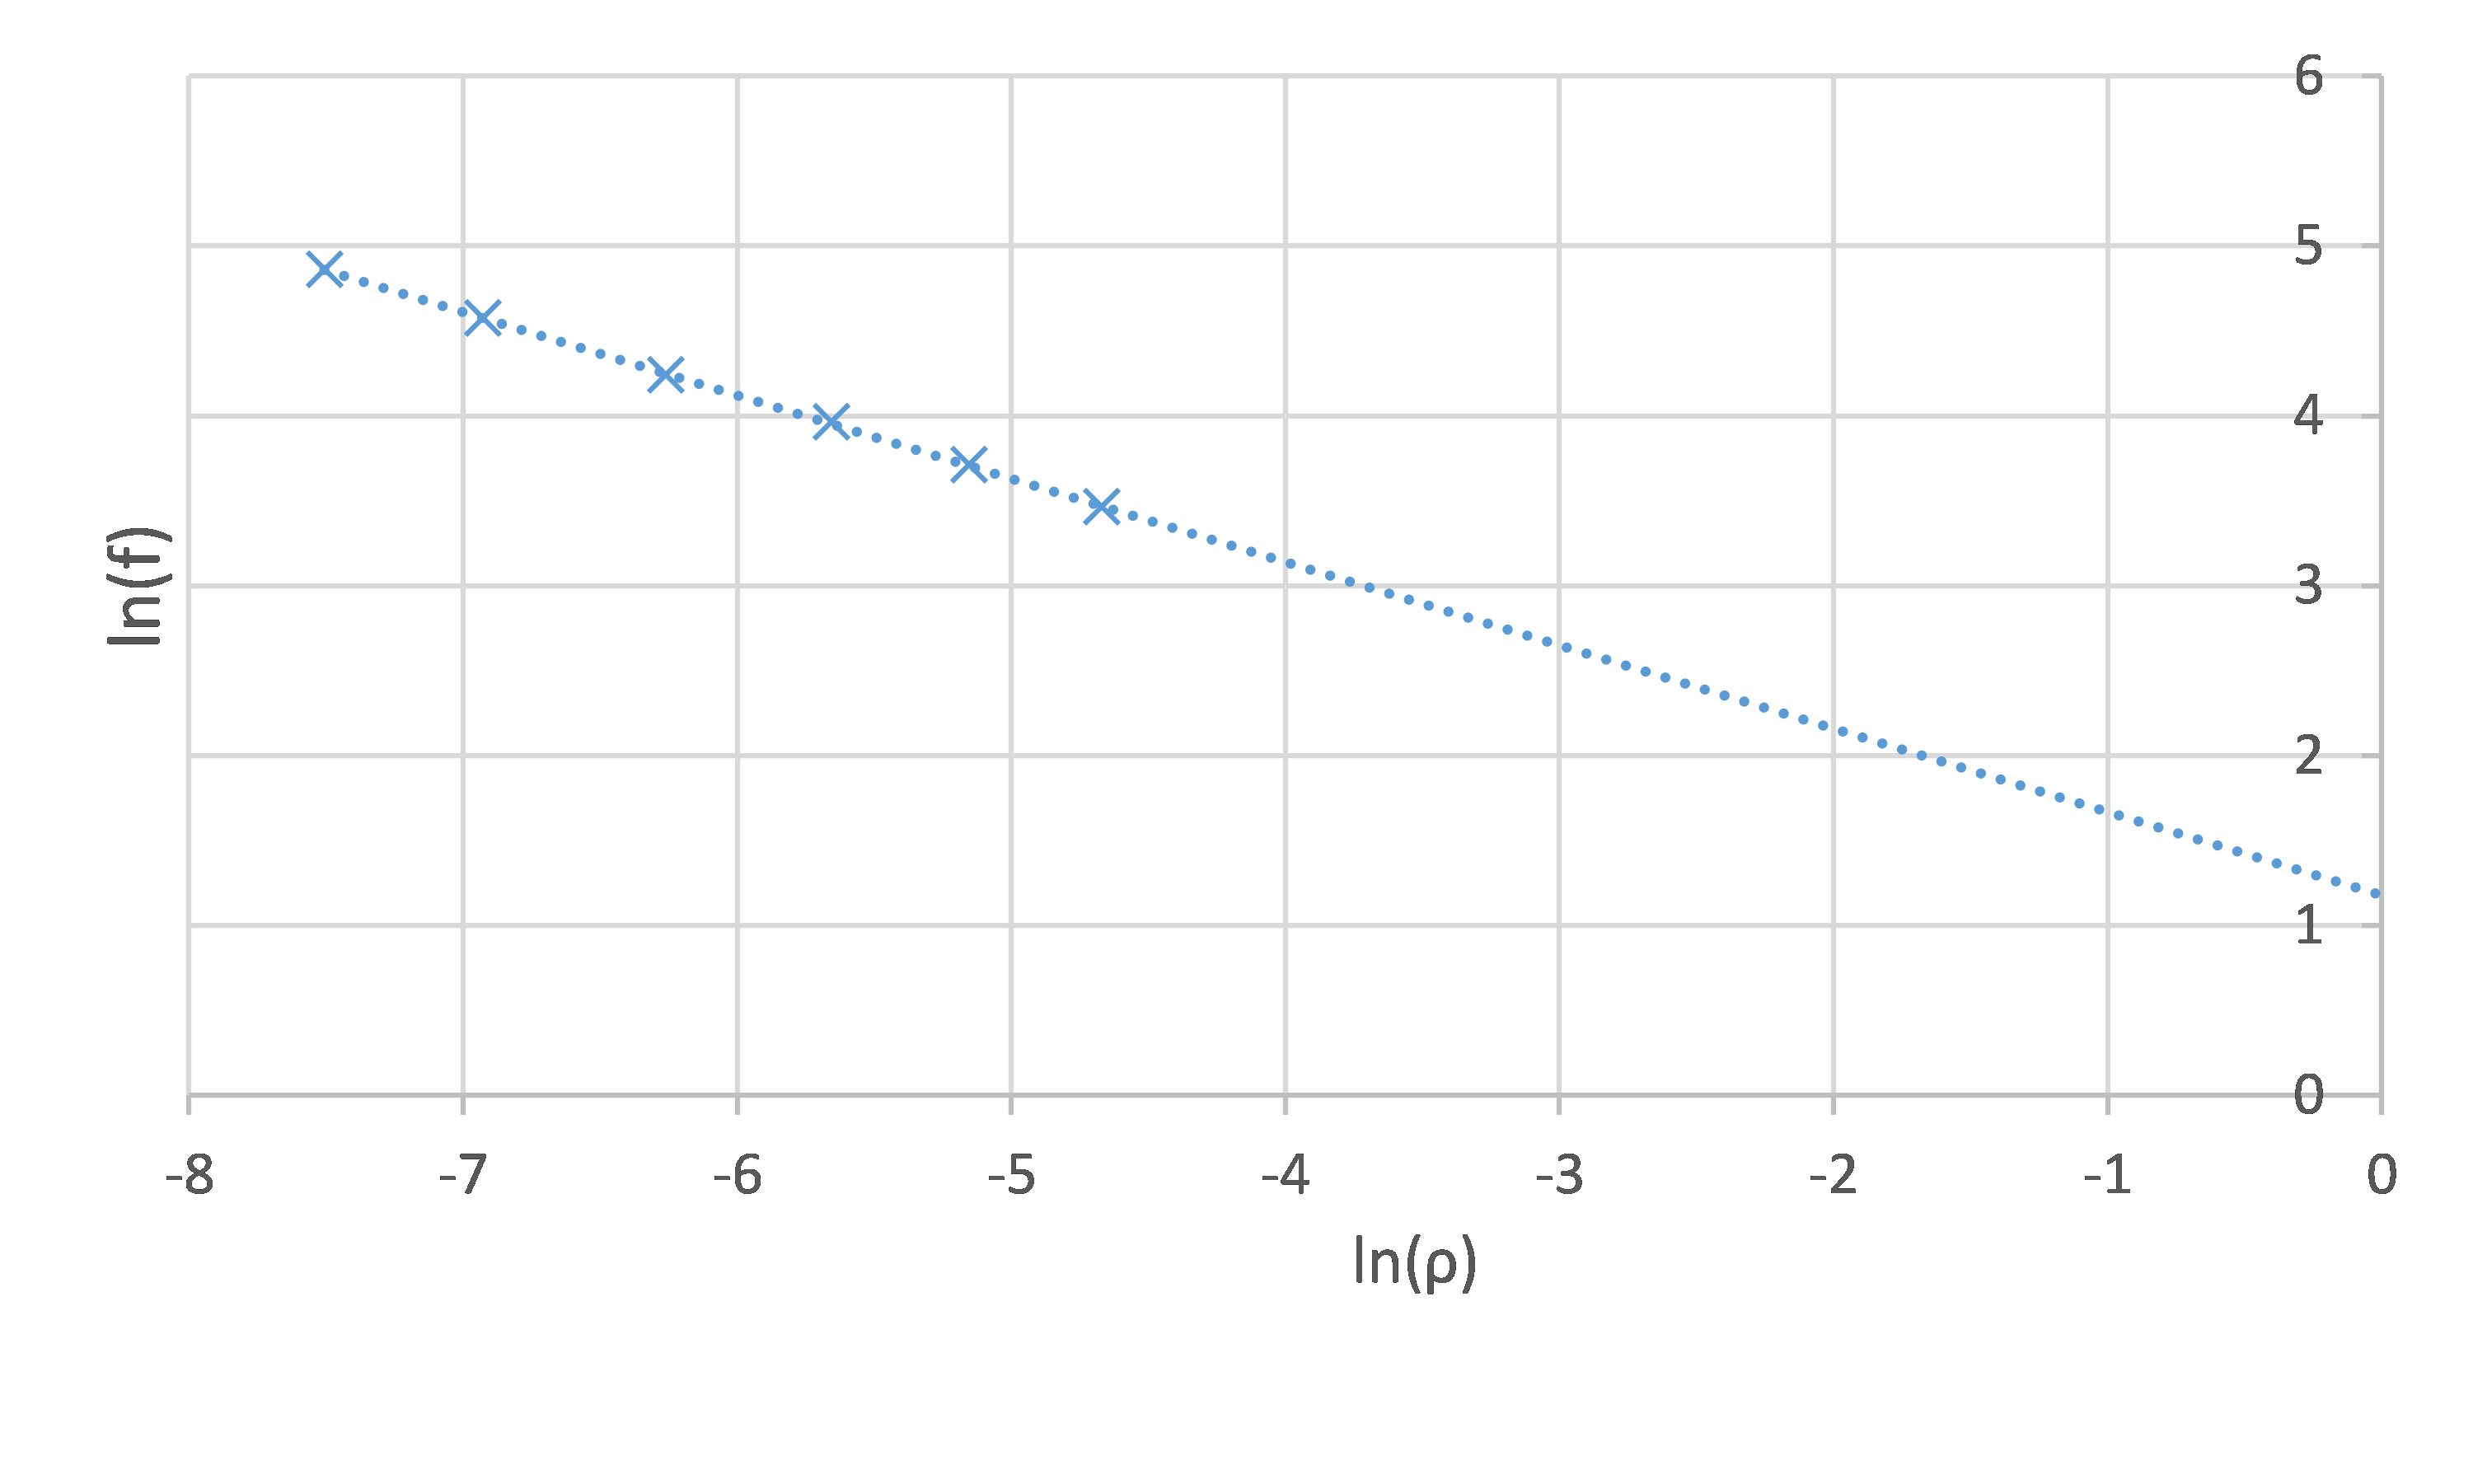
\includegraphics[scale=0.15]{7.png}
\caption{1\#--6\#弦线$ln(f)$与$ln(\rho)$关系图}}
\end{figure}
拟合直线斜率的相对不确定度$\frac{k}{U_k} = 2\%$,截距的相对不确定度$\frac{b}{U_b} = 5\%$,表明f与n的线性关系较好. 计算理论斜率与截距,直线理论斜率应为$k_0=-0.500$,理论截距应为$b_0=lnn-ln(2L)+\frac{1}{2}ln(T)=1.141$,可见实验得出的斜率和截距与理论数值也比较接近.


\subsubsection*{E) 分析弦的线密度、弦长、张力、基频与波速的关系}
通过采用前述C)获得的数据,2\#和1\#弦线上拉力改变时,可以通过$v=f\lambda=\frac{2L}{n}f$计算出弦上振动传播速度的实验值,而理论值可由$v=\sqrt{\frac{T}{\rho}}$计算出. 可以通过比较相对误差大小,衡量出实验值与理论值的差距,检验实验数据的正确性.
为了衡量相对误差的大小,设理论值为$\mu$,实验值为$x$,则可定义相对误差:
\begin{equation}
E=\big{|}\frac{x-\mu}{\mu}\big{|}\times100\%
\end{equation}\par
\paragraph{对于2\#弦线的数据分析如下:}
\begin{center}
{\kaishu 表8 2\#弦线的实验数据表($L=50.00cm, n=1, \rho=0.00098kg/m$)}
\begin{tabular}{|c|c|c|c|c|c|c|}
\hline
	$F/N$&1.960&3.920&5.880&7.840&9.800&11.760\\
\hline
	$f/Hz$&43.24&59.67&74.57&87.17&97.01&105.67\\
\hline
	实验值$\hat{v}/(m\cdot s^{-1})$&43.24&59.67&74.57&87.17&97.01&105.67\\
\hline
	理论值${v_0}/(m\cdot s^{-1})$&44.72&63.25&77.46&89.44&100.00&109.54\\
\hline
	相对误差E&3\%&5\%&4\%&3\%&3\%&4\%\\
\hline
\end{tabular}\end{center}\par
观察上述一组数据,相对误差均在5\%以内,可见实验值和理论值吻合较好.

\paragraph{对于1\#弦线的数据分析如下:}
\begin{center}
{\kaishu 表8 2\#弦线的实验数据表($L=50.00cm, n=1, \rho=0.00055kg/m$)}
\begin{tabular}{|c|c|c|c|c|c|c|}
\hline
	$F/N$&1.960&3.920&5.880&7.840&9.800&11.760\\
\hline
	$f/Hz$&57.51&81.65&99.77&115.56&129.47&140.91\\
\hline
	实验值$\hat{v}/(m\cdot s^{-1})$&57.51&81.65&99.77&115.56&129.47&140.91\\
\hline
	理论值${v_0}/(m\cdot s^{-1})$&59.70&84.42&103.40&119.39&133.49&146.22\\
\hline
	相对误差E&4\%&3\%&4\%&3\%&3\%&4\%\\
\hline
\end{tabular}\end{center}\par
观察上述一组数据,相对误差均在5\%以内,可见实验值和理论值吻合较好.

\section{思考题}
\subsubsection*{A) 为了方便地激发和测量弦振动现象,激励线圈和探测线圈应如何放置?}
\paragraph{1.}根据当前实验条件下会产生的半波数$n$,估测形成驻波时波节和波腹大致会出现的位置. 大致来说,以最左端弦码为$x=0cm$处,则波节在$x=\frac{mL}{n}(m=1,2,\cdots,n-1)$处,波腹在$x=\frac{mL}{2n}(m=1,3,\cdots,2n-1)$处. 进行实验时,要将\textbf{探测线圈大概放置于波腹所在位置},以保证接收到的波振幅更大,更易观测出振幅变化.
\paragraph{2.}两个线圈距离过近时会发生互感现象,信号相互干扰,造成较大的实验误差,因此\textbf{激励线圈和探测线圈应至少保持10cm的距离}.

\subsubsection*{B) 如何快速找到一定实验条件下弦振动的共振频率?}
\paragraph{1.}\textbf{先用计算器算出当前条件下共振频率的理论数值,在低于此理论值的一定数值时开始调节,将发生器信号频率缓缓提高},观察屏幕上$CH2$的振幅变化. 若振幅变大,则共振频率大于当前频率;若振幅变小,则共振频率小于当前频率,通过这种方法找到共振频率大致范围.
\paragraph{2.}\textbf{调节信号频率时速度要缓慢},共振的能量积累需要一定过程. 改变信号频率后,$CH2$的图形变化会非常缓慢,若频率调节过快,则极有可能错过共振频率点.
\paragraph{3.}\textbf{初始调节频率时,可将$CH2$的垂直偏转因子调小},以便及时观察到波形的微小变化. 在共振频率附近,$CH2$图像的振幅会增大,可及时适当增大$CH2$的垂直偏转因子,以保证屏幕中可以显示出正弦图像的峰值,完整体现出振幅的变化.
\paragraph{4.}在共振频率附近,可以\textbf{打开光标辅助测量},将光标调节至与正弦图像相切之处,微调信号源频率,稍等片刻查看峰值是否超越光标横线. 若超过则说明更加靠近共振频率,反之则是远离.
\paragraph{5.}调节发生器信号频率时,要采取\textbf{先粗调再细调}的方式,先以大步进值调节寻找出现正弦波形的发生器信号频率范围,确定大致范围后再精细调节更小步进值的频率,以快速找到共振频率.

\section{讨论与分析}
\paragraph{1.}注意可以根据实验条件调整合适的信号$V_{pp}$数值,数值过大时弦线抖动过于剧烈(在基频频率时尤其需要控制调小$V_{pp}$),信号接收器的磁通变化过大,导致模拟出的信号出现较大误差,从而在示波器上显现不正确的图形,同时,过强抖动也有可能使弦线吸附到接收器上(信号接收器具有一定磁性,应时刻注意弦线是否被信号接收器吸附,从而在示波器上产生不可辨认的粗糙直线图形),况且过大的抖动可能会使弦的振动不满足小角近似,导致弦振动方程产生误差. 而信号$V_{pp}$数值过小时,示波器上振幅不明显,不易进行观测,从而不易找到共振频率.
\paragraph{2.}在实验中,有一个问题值得思考:拉力的变化是否会引起弦线发生应变,进而引起密度变化,导致测量误差呢?对此我认为有必要进行如下计算说明:
在估测中权且仅进行数量级的估计,对此,取弦上张力$F$数量级为$10N$,目测弦线半径$r$数量级为$10^{-3}m$,总长度L数量级为$1m$,根据弦线为金属材料,可取杨氏模量$E$为$10^11Pa$数量级,则由杨氏模量的定义$E=\frac{F\cdot L}{S\cdot \Delta L}$,有
\[\Delta L = \frac{F\cdot L}{S\cdot E} = \frac{F\cdot L}{\pi r^2\cdot E}\sim10^{-4}m\sim1mm\]
相对变化量$\frac{\Delta L}{L}\sim10^{-4}$,此量小到可以被忽略不计.
\paragraph{3.}不同实验条件采用不同密度的弦线是为了共振频率分布在合理范围.\par 对于实验A),采用较粗的6\#和5\#弦线,在$n=5$条件下共振频率的理论值分别为$160Hz$和$210Hz$左右,此时若采用较细的2\#和1\#弦线,共振频率将达到$350Hz$和$660Hz$,这么高的频率会导致共振频率的寻找范围变大,且灵敏度会变小,使得共振频率更难被测得,也可能导致数据有效位数的降低;而且此种情况下探测线圈磁通变化过大,可能引起接收信号失真等问题.\par
对于实验B),采用较细的2\#和1\#弦线,在$T=1.960N$条件下共振频率的理论值分别约为$40Hz$和$60Hz$,此时若采用较粗的6\#和5\#弦线,共振频率将降为大约$15Hz$和$18Hz$,这么低的频率会使得寻找共振频率异常困难,信号源微小的频率变化都有可能导致振幅极大的波动,分度值过大,灵敏度过高,甚至有可能导致找不到合适的共振频率.\par
对于实验C),若采用的弦线过粗或过细,都有可能导致共振频率不在合适的范围,内容大体同上,不再赘述.
\paragraph{4.}示波器上显示$CH1$的原因:\par
既然$CH1$与形成驻波时$CH2$的振幅完全不同,则为什么要在示波器上显示$CH1$的波形呢?我认为,这是因为$CH1$与$CH2$的频率大致相等,显示完整清晰的$CH1$波形有助于调整示波器合适的水平偏转因子数值,以便更好地显示驻波振动图像,找到共振频率.

\paragraph{5.}可能导致误差的因素:\par
\textbf{i.)} 弦振动方程的建立运用多处近似,当弦线振动幅度较大时,就可能出现较大误差;而且该模型是通过理想轻绳建立的模型,现实中弦线必然会有质量,受重力影响也可能产生误差; \textbf{ii.)} 探测线圈探测到的信号存在偏差,甚至在某些条件下波形都不是光滑的正弦波形,而是存在许多噪声,在实验观测过程中能够明显感受到这一点;
\textbf{iii.)} 砝码直接手触,会有磨损,质量会有偏差;重力加速度近似为$9.8m/s^2$,并没有通过实验测量,也存在一定误差; \textbf{ix.)} 信号发生器和弦线接收到的频率不一定相等,在传输过程中可能会有误差,这一点在示波器的频率显示上有所体现; \textbf{x.)} 滑轮与细绳之间存在摩擦力,且弦码和弦线间可能存在摩擦力、支持力等多种作用力,使得弦线上张力并不一定等于理论值; \textbf{xi.)} 弦码存在一定厚度,且肉眼可见,由于长久使用,弦码被弦线磨出凹槽,使得弦线不能很好被弦码固定。这不但会导致$L$发生变化,更有可能使得边界条件发生变化,使反射波的产生并不符合该题的理论计算; \textbf{xii.)} 刚将砝码钩挂在细线上时,砝码摆动会对测量造成一定困难(可用手扶住钩码待其缓缓静止后松开,再进行试验),同时,风的吹动、桌子的晃动甚至身边同学的走动都会给实验的测量带来误差. \textbf{xiii.)} 给定的弦线密度可能也会有偏差\par
以上均为系统误差,实验过程中,各数据均为单次测量,也难免会因为人为因素而产生随机误差. 因此,综合考虑以上因素,本次实验的测量数据与理论值吻合得较好.

\section{实验结论}
	在该实验中,我们主要通过测量弦线上驻波的共振频率,验证了有关于弦线上振动传播和反射、弦线上驻波产生条件等相关知识.\par
	具体说来,我们通过理论推导共振频率$\displaystyle{f = \frac{n}{2L}\sqrt{\frac{T}{\rho}}}$,得知$f$仅与$n$、$L$、$T$、$\rho$四个变量有关,因此采用控制变量法,分别使单一变量变化,从而探究这些变量与$f$的关系. 之后,我们通过弦上振动传播速度的两个不同计算方法,将测量数据得出的实验值与理论值做横向比较,发现二者吻合较好,验证了实验原理和本次实验操作的正确性.\par
	在进行本次试验过程中,我初步掌握了进行物理实验的步骤和基本方法,了解到了实验过程中是如何进行测量、记录、排除干扰等各项工作的。在后续处理数据、撰写实验报告的过程中,我还系统性地掌握了实验误差的分析、不确定度的计算、直线拟合等相关知识,并对Latex、Excel等工具的掌握程度有了进一步提高.
\newpage
\section{原始数据}
\begin{figure}[hb]\centering{
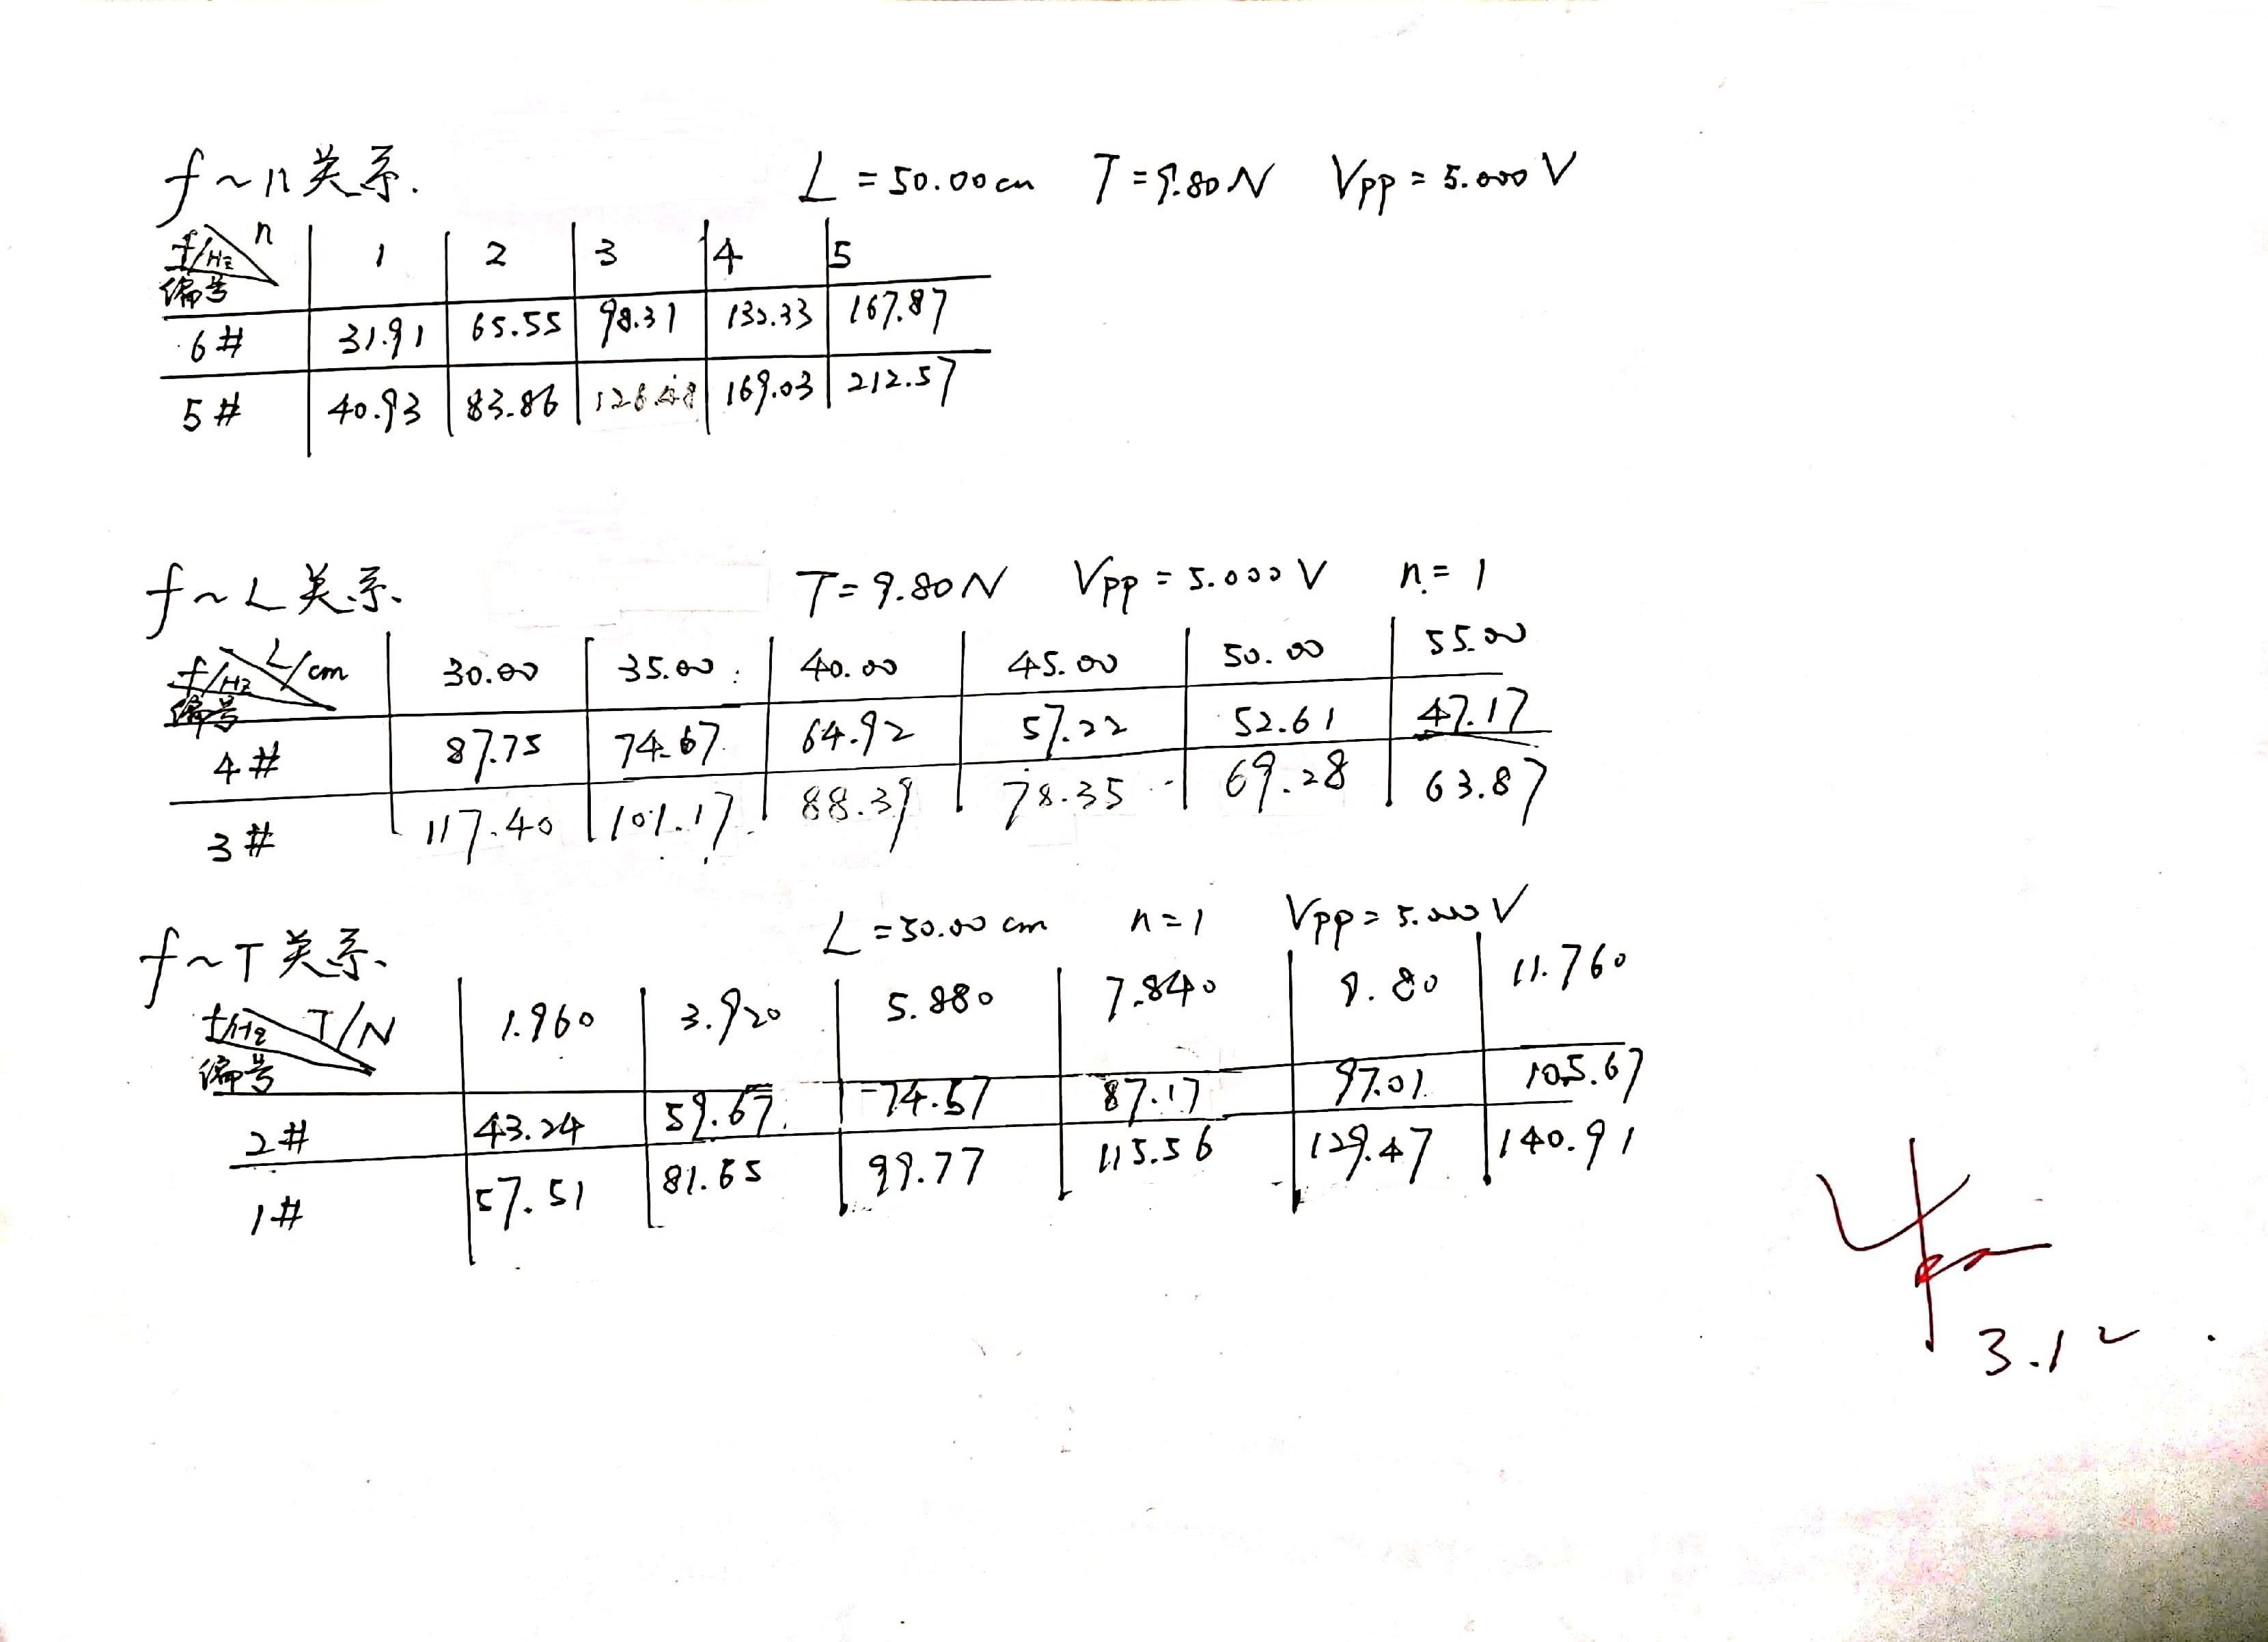
\includegraphics[scale=0.23]{0.jpg}}
\end{figure}
\end{document}